%\documentclass[sigconf, anonymous]{acmart}
\documentclass[conference]{IEEEtran}
%\usepackage[utf8]{inputenc}


%% 1. usepackage should go into "usepackages.tex"
%% 2. newcommand should be defined in "newcommands.tex"
% This is to fix the problem of IEEEtran. 
% \labelindent command exists for legacy reasons in the IEEE template.
%\let\labelindent\relax

% CY: for customizing item symbols.

\usepackage[inline]{enumitem}

\usepackage[english]{babel}
\usepackage[utf8]{inputenc}
\usepackage{amsthm} % for proof
\usepackage{amsmath}
\usepackage{graphicx}
\usepackage{boxedminipage}
\usepackage{epsfig}
\usepackage{psfrag}
\usepackage{url}
\usepackage{comment}
\usepackage{afterpage}
%\usepackage{cite}
\usepackage{pstricks}
\usepackage{graphics}

% #### CY: I disable mathenv for enabling tabularx
%\usepackage{mathenv}

\usepackage{mdwtab}
%\usepackage{floatflt}
\usepackage{wrapfig}
\usepackage{graphics}

\usepackage{algorithm}  
\usepackage{algorithmic} 
%\usepackage{algorithmicx}
%\usepackage{algpseudocode}
%\usepackage{algpseudocode}

%\algdef{SE}[DOWHILE]{Do}{doWhile}{\algorithmicdo}[1]{\algorithmicwhile\ #1}%
%\usepackage[linesnumbered, ruled]{algorithm2e}
%\SetKwRepeat{Do}{do}{while}

% Added by CY
%\usepackage{algpseudocode}
\usepackage{amssymb} % for \triangleq denotation in the appendix

% CY: for multi-line in tables
\usepackage{makecell}


% CY: for double line in tables
\usepackage{hhline}

% CY: for easier making tables
\usepackage{tabularx}

% CY: for colorful table.
%\usepackage[table,xcdraw]{xcolor}

% For hyperlink
\usepackage{hyperref}

\usepackage{epsfig}
%\usepackage{caption}
\usepackage{fixfoot}
%\usepackage{footmisc}
%\usepackage{enumitem}
\usepackage{listings}
\usepackage{psfrag,wrapfig}
\usepackage{xspace,soul}
%\usepackage[small,compact]{titlesec}
%\usepackage[disable]{todonotes}
\usepackage[colorinlistoftodos]{todonotes}
%\usepackage{palatino}

% This package is for fixing "! No room for a new \dimen ." error. by CY
%\usepackage{etex}


%\usepackage{subfigure}	% CY: this is deprecated. Use subcaption instead
% This package is for \captionsetup used in figures.
%\usepackage{caption}
\usepackage{subcaption}

% CY: for figure and table side by side 
% \usepackage{floatrow}
% % Table float box with bottom caption, box width adjusted to content
% \newfloatcommand{capbtabbox}{table}[][\FBwidth]

%% --------------------- Start Some definitions to make life easier -----------------------------
\newcommand{\da}{\downarrow}
\newcommand{\la}{\leftarrow}
\newcommand{\ra}{\rightarrow}
\newcommand{\lla}{\longleftarrow}
\newcommand{\llra}{\longleftrightarrow}
\newcommand{\lra}{\longrightarrow}
\newcommand{\Lla}{\Longleftarrow}
\newcommand{\Llra}{\Longleftrightarrow}
\newcommand{\Lra}{\Longrightarrow}
\newcommand{\ua}{\uparrow}

\newcommand{\nea}{\nearrow}
\newcommand{\nwa}{\nwarrow}
\newcommand{\sea}{\searrow}
\newcommand{\swa}{\swarrow}

\newcommand{\mf}{\mathbf}
\newcommand{\mc}{\mathcal}
\newcommand{\mi}{\mathit}
%\newcommand{\ul}{\underline}
\newcommand{\ol}{\overline}

\newcommand{\eg}{{\it e.g.,}\xspace}
\newcommand{\viz}{{\it viz.,}}
\newcommand{\Eg}{{\it E.g., }}
\newcommand{\etal}{{\it et~al.}}
\newcommand{\ie}{{\it i.e.,}\xspace}
\newcommand{\Ie}{I.e.,\xspace}
\newcommand{\etc}{{\it etc.~}}
\newcommand{\ci}{{\it (i) }}
\newcommand{\cii}{{\it (ii) }}
\newcommand{\ciii}{{\it (iii) }}
\newcommand{\civ}{{\it (iv) }}
\newcommand{\cv}{{\it (v) }}
\newcommand{\cvi}{{\it (vi) }}
\newcommand{\ca}{{\it (a) }}
\newcommand{\cb}{{\it (b) }}
\newcommand{\cc}{{\it (c) }}
\newcommand{\cd}{{\it (d) }}
\newcommand{\ce}{{\it (e) }}
\newcommand{\cf}{{\it (f) }}
\newcommand{\cg}{{\it (g) }}
\newcommand{\ch}{{\it (h) }}
%\newcommand{\ci}{{\it (i) }}
\newcommand{\cj}{{\it (j) }}
\newcommand{\ck}{{\it (k) }}
\newcommand{\cl}{{\it (l) }}
\newcommand{\cm}{{\it (m) }}
\newcommand{\cn}{{\it (n) }}
\newcommand{\co}{{\it (o) }}
\newcommand{\cp}{{\it (p) }}
\newcommand{\cq}{{\it (q) }}
\newcommand{\Note}{{\bf Note: }}

% CY: This is for the Example items.
%\usepackage{amsthm}
%\theoremstyle{definition}
\newtheorem{definition}{Definition}
\newtheorem{example}{Example}
%\setcounter{example}{1}
%\newtheorem{remark}{Remark}
%\newtheorem{corollary}{Corollary}
%\newtheorem{lemma}{Lemma}
%\newtheorem{principle}[definition]{Principle}
%\newtheorem{proposition}[definition]{Proposition}
\newtheorem{theorem}{Theorem}
\newtheorem{observation}{Observation}

% CY: to make the square solid
\renewcommand{\qedsymbol}{$\blacksquare$}

% This is for supporting algorithm lines without showing line numbers.
\newcommand\StateX{\Statex\hspace{\algorithmicindent}}


%%%%% Commands added by Potok %%%%%
% Operations
\newcommand{\OP}{\mathit{OP}}
\newcommand{\OPALL}{\overline{\OP}}
\newcommand{\op}{\mathit{op}}
\newcommand{\optop}{\op_\top}
\newcommand{\opbot}{\op_\bot}
\newcommand{\move}{\mathit{move}}
\newcommand{\transfer}{\mathit{transfer}}
\newcommand{\noop}{\mathit{noop}}

% Cells
\newcommand{\verttop}{\mathit{v}_\top}
\newcommand{\vertbot}{\mathit{v}_\bot}

% Widgets
\newcommand{\Wtop}{\mathit{W}_\top}
\newcommand{\Wbot}{\mathit{W}_\bot}
\newcommand{\Word}{\mathit{W}_\circ}

% Plant functions
\newcommand{\Lmap}{\mathit{L}}
\newcommand{\Tmap}{\mathit{T}}
\newcommand{\Qmap}{\mathit{Q}}
\newcommand{\Rmap}{\mathit{R}}

% Plant variables
\newcommand{\loc}{\mathit{loc}}
\newcommand{\pos}{\mathit{pos}}
\newcommand{\status}{\mathit{status}}
\newcommand{\queue}{\mathit{queue}}
\newcommand{\timer}{\mathit{timer}}
\newcommand{\operational}{\mathit{operational}}
\newcommand{\idle}{\mathit{idle}}
\newcommand{\waiting}{\mathit{waiting}}

% Miscellaneous operations/variables
\newcommand{\head}{\mathit{head}}
\newcommand{\pop}{\mathit{pop}}
\newcommand{\len}{\mathit{len}}
\newcommand{\prev}{\mathit{prev}}
\newcommand{\bag}{\mathit{bag}}
\newcommand{\Bag}{\mathit{Bag}}
\newcommand{\trytransfer}{\mathit{try\_transfer}}

% Controller variables
\newcommand{\action}{\mathit{action}}
\newcommand{\celltype}{\mathit{celltype}}
\newcommand{\completed}{\mathit{completed}}
\newcommand{\cost}{\mathit{cost}}
\newcommand{\nexttr}{\mathit{next\_tr}}
\newcommand{\req}{\mathit{requirement}}
\newcommand{\starttime}{\mathit{start\_time}}
\newcommand{\canenqueue}{\mathit{can\_enqueue}}
\newcommand{\waittime}{\mathit{wait\_time}}
\newcommand{\widgettime}{\mathit{widget\_time}}
\newcommand{\ptr}{\mathit{pointer}}

% General
\newcommand{\True}{\mathsf{T}}
\newcommand{\False}{\mathsf{F}}
\newcommand{\potok}[1]{\textcolor{teal}{#1}}
\newcommand{\cy}[1]{\textcolor{brown}{#1}}
\newcommand{\rednote}[1]{\textcolor{red}{#1}}

% Plan
\newcommand{\plan}{\mathit{C}}
\newcommand{\mfname}{SDCWorks\xspace}

%\usepackage{paralist}
% marking changes

%\newcommand{\mitras}[1]{\textcolor{blue}{#1}}
\newcommand{\mitras}[1]{{#1}}
% for nomencl to produce page links
%\renewcommand*{\pagedeclaration}[1]{\unskip, \hyperpage{#1}}
%\renewcommand{\nomname}{List of Symbols and Functions}

\newcommand{\authcomment}[1]{\textbf{[[#1]]}}
%\newcommand{\sayan}[1]{\textcolor{blue}{\textbf{[SM: [#1]]}}}
%\newcommand{\taylor}[1]{\textcolor{red}{\textbf{[TJ: [#1]]}}}

\newcommand{\revision}[1]{\textcolor{blue}{#1}}

% blank all comments
\newcommand{\sayan}[1]{\textcolor{blue}{#1}}

%FIXED SETS

%\newcommand{\Time}{{\sf T}}                     %time domain
\newcommand{\nnt}{{\sf T}^{\geq 0}}             %nonnegative time points
\newcommand{\post}{{\sf T}^{>0}}                %positive time points
\newcommand{\Variables}{{\sf V}}                %variables

\newcommand{\num}[1]{\relax\ifmmode \mathbb #1\else $\mathbb #1$\fi}
\newcommand{\nnnum}[1]{\relax\ifmmode 
  {\mathbb #1}_{\geq 0} \else ${\mathbb #1}_{\geq 0}$
  \fi}
\newcommand{\npnum}[1]{\relax\ifmmode 
  {\mathbb #1}_{\leq 0} \else ${\mathbb #1}_{\leq 0}$
  \fi}
\newcommand{\pnum}[1]{\relax\ifmmode 
  {\mathbb #1}_{> 0} \else ${\mathbb #1}_{> 0}$
  \fi}
\newcommand{\nnum}[1]{\relax\ifmmode 
  {\mathbb #1}_{< 0} \else ${\mathbb #1}_{< 0}$
  \fi}
\newcommand{\plnum}[1]{\relax\ifmmode 
  {\mathbb #1}_{+} \else ${\mathbb #1}_{+}$
  \fi}
\newcommand{\nenum}[1]{\relax\ifmmode 
  {\mathbb #1}_{-} \else ${\mathbb #1}_{-}$
  \fi}

\newcommand{\reals}{{\num R}}                    %reals
\newcommand{\booleans}{{\num B}}                    %reals
\newcommand{\nnreals}{{\nnnum R}}                    %nonnegative reals
\newcommand{\realsinfty}{{\num R} \cup \{\infty, -\infty\}}                    %nonnegative reals
\newcommand{\plreals}{{\plnum R}}                    %positive reals
\newcommand{\naturals}{{\num N}}                      %natural numbers
\newcommand{\integers}{{\num Z}}                      %integers
\newcommand{\rationals}{{\num Q}}                      %rationals
\newcommand{\nnrationals}{{\nnnum Q}}                   % nonnegative rationals
\newcommand{\Time}{{\num T}}  

% EXECUTIONS TRACES and FRAGS
\newcommand{\extb}[1]{\relax\ifmmode {\sf ExtBeh}_{#1} \else ${\sf ExtBeh}_{#1}$\fi} 
\newcommand{\tdists}[1]{\relax\ifmmode {\sf Tdists}_{#1} \else ${\sf Tdists}_{#1}$\fi} 

\newcommand{\exec}[1]{\relax\ifmmode {\sf Execs}_{#1} \else ${\sf Exec}_{#1}$\fi} 
\newcommand{\execf}[1]{\relax\ifmmode {\sf Execs}^*_{#1} \else ${\sf Exec}^*_{#1}$\fi} 
\newcommand{\execi}[1]{\relax\ifmmode {\sf Execs}^\omega_{#1} \else ${\sf Exec}^\omega_{#1}$\fi} 

\newcommand{\ctrace}[1]{\relax\ifmmode {\sf Ctraces}_{#1} \else ${\sf Ctraces}_{#1}$\fi} 

\newcommand{\trace}[1]{\relax\ifmmode {\sf Traces}_{#1} \else ${\sf Traces}_{#1}$\fi} 
\newcommand{\tracef}[1]{\relax\ifmmode {\sf Traces}^*_{#1} \else ${\sf Traces}^*_{#1}$\fi} 
\newcommand{\tracei}[1]{\relax\ifmmode {\sf Traces}^\omega_{#1} \else ${\sf Traces}^\omega_{#1}$\fi} 

\newcommand{\frag}[1]{\relax\ifmmode {\sf Frags}_{#1} \else ${\sf Frags}_{#1}$\fi} 
\newcommand{\fragf}[1]{\relax\ifmmode {\sf Frags}^*_{#1} \else ${\sf Frags}^*_{#1}$\fi} 
\newcommand{\fragi}[1]{\relax\ifmmode {\sf Frags}^\omega_{#1} \else ${\sf Frags}^\omega_{#1}$\fi} 

\newcommand{\reach}[1]{\relax\ifmmode {\sf Reach}_{#1} \else ${\sf Reach}_{#1}$\fi} 

\newcommand{\execs}{{\exec{}}}
\newcommand{\traces}{{\trace{}}}
\newcommand{\fragss}{{\frag{}}}

\newcommand{\fexecs}{{\execf{}}}
\newcommand{\ftraces}{{\tracef{}}}
\newcommand{\ffragss}{{\fragf{}}}

\newcommand{\iexecs}{{\execi{}}}
\newcommand{\itraces}{{\tracei{}}}
\newcommand{\ifragss}{{\fragi{}}}


\newenvironment{noqedproof}{\pf}{}
%\newcommand{\pf}{\par\noindent{\bf Proof:}~}


% \newcounter{theorem}
%%\renewcommand{\thesubsection}{\arabic{subsection}}
\newtheorem{rtheorem}{Theorem}
\newtheorem{lemma}[theorem]{Lemma}
\newtheorem{corollary}[theorem]{Corollary}
\newtheorem{claim}[theorem]{Claim}
%\theoremstyle{definition}
% \newtheorem{definition}{Definition}[section]
% \renewcommand{\qed}{\hfill{\rule{2mm}{2mm}}\medskip}
%% \newenvironment{proof}{\pf}{\qed}
\newtheorem{proposition}[theorem]{Proposition}
\newtheorem{inv}[theorem]{Invariant}
\newcounter{assump}
\newtheorem{assumption}[assump]{Assumption}
% \newtheorem{remark}[theorem]{Remark}
%%\theoremstyle{assumption}
% \newtheorem{assumption}{Assumption}[section]

 
 %\newenvironment{example}
 %{\refstepcounter{theorem} \vspace{2ex}\par\noindent
 %\textbf{Example}~\textbf{\thetheorem~}}{\qed}
 
%\theoremstyle{remark}
% \newcounter{example}
% \newtheorem{example}{Example}[chapter]
% {\refstepcounter{theorem} \vspace{2ex}\par\noindent
% \textbf{Example}~\textbf{\theexampletheorem~}}{\qed}
 
 
 \def\examplenonum#1#2{
	\vspace{.15in}
	\noindent
	{\bf Example #1}{\em ~(continued)}{\bf .}
	{#2}{\qed}
	}
% 
% \renewcommand{\theequation}{\thesection.\arabic{equation}}
% \renewcommand{\thefigure}{\thesection.\arabic{figure}}
% \renewcommand{\thetable}{\thesection.\arabic{table}}
% \newcommand{\Section}[1]{\section{#1}%
%    \setcounter{equation}{0}\setcounter{figure}{0}\setcounter{table}{0}%
%    \setcounter{example}{0}}
% 
% \newenvironment{anotation}[1][Nancy]{\begin{quote}\small[[[#1]]]}{\normalsize\end{quote}}
% \newcommand{\ba}{\begin{anotation}}
% \newcommand{\ea}{\end{anotation}}
% 
% \newcommand{\bcb}{\chgbarbegin}
% \newcommand{\ecb}{\chgbarend}
% \chgbarwidth 1pt
% 
% \newcommand{\dec}{\ensuremath{{:}}}
% \newcommand{\eqdef}{\mathbin{::=}}
% \newcommand{\I}{{\ensuremath{\cap}}}



% OPERATIONS ON SETS, RELATIONS AND FUNCTIONS
\newcommand{\pow}[1]{{\bf P}(#1)} % powerset
\newcommand{\inverse}[1]{#1^{-1}}
\newcommand{\range}[1]{\ms{range{(#1)}}}
\newcommand{\domain}[1]{{\it dom}(#1)}
\newcommand{\type}[1]{\ms{type{(#1)}}}
\newcommand{\dtype}[1]{\ms{dtype{(#1)}}} % dynamic type
\newcommand{\restr}{\mathrel{\lceil}}
\newcommand{\proj}{\matrel{\lceil}}
\newcommand{\restrrange}{\mathrel{\downarrow}}
\newcommand{\point}[1]{\wp(#1)}     		%point trajectory



% HYBRID AUTOMATA
\def\A{{\cal A}} % HA
\def\B{{\cal B}} % HA
\def\C{{\cal C}} % HA
\def\D{{\cal D}} % set of discrete steps
\def\E{{\cal E}} % HA
\def\F{{\cal F}} % HA
\def\G{{\cal G}} % pieces of SHIOA
\def\H{{\cal H}} % HA
\def\I{{\cal I}} % environment sequence
\def\K{{\cal K}} % environment sequence
\def\M{{\cal M}} % Mode switching transitions
\def\O{{\cal O}} % outcome function
\def\P{{\cal P}} % set of modes
\def\Q{{\cal Q}} % set of modes
\def\R{{\cal R}} % relation
\def\S{{\cal S}} % set of trajectories
\def\T{{\cal T}} % set of trajectories
\def\V{{\cal V}} % Lyapunov function
\def\U{{\cal U}} % set of trajectories
\def\X{{\cal X}} % Lyapunov function
\def\Y{{\cal Y}} % set of trajectories


% more special characters

\newcommand{\col}[1]{\relax\ifmmode \mathscr #1\else $\mathscr #1$\fi}

\def\statemodels{\col{S}}


% Names of actions, automata etc
%\definecolor{HIOAcolor}{rgb}{0.776,0.22,0.07}
%\newcommand{\HIOA}{\textcolor{HIOAcolor}{\tt HIOA\hspace{3pt}}}
%\newcommand{\PVS}{\textcolor{HIOAcolor}{\tt PVS\hspace{3pt}}}
%\newcommand{\PVSnogap}{\textcolor{HIOAcolor}{\tt PVS\hspace{1pt}}}
%\newcommand{\HIOAbiggap}{\textcolor{HIOAcolor}{\tt HIOA\hspace{6pt}}}
%\newcommand{\HIOAnogap}{\textcolor{HIOAcolor}{\tt HIOA}}
%\newcommand{\anyrelation}{\lessgtr}

% Transformation for ADT
\newcommand{\SC}[2]{\relax\ifmmode {\tt Scount}(#1,#2) \else ${\tt Scount}(#1,#2)$\fi} 
\newcommand{\SCM}[2]{\relax\ifmmode {\tt Smin}(#1,#2) \else ${\tt Smin}(#1,#2)$\fi} 
\newcommand{\Aut}[1]{\relax\ifmmode {\tt Aut}(#1) \else ${\tt Aut}(#1)$\fi} 

\newcommand{\auto}[1]{{\operatorname{\mathsf{#1}}}}
\newcommand{\act}[1]{{\operatorname{\mathsf{#1}}}}
\newcommand{\smodel}[1]{{\operatorname{\mathsf{#1}}}}
\newcommand{\pvstheory}[1]{{\operatorname{\mathit{#1}}}}
%\newcommand{\auto}[1]{\relax\ifmmode \sf #1\else $\sf #1$\fi}
%\newcommand{\act}[1]{\relax\ifmmode \sf #1\else $\sf #1$\fi}


\newcommand{\Automaton}{{\bf automaton}}
\newcommand{\Asserts}{{\bf asserts}}
\newcommand{\Assumes}{{\bf assumes}}
\newcommand{\Backward}{{\bf backward}}
\newcommand{\By}{{\bf by}}
%\newcommand{\Case}{{\bf case}}
\newcommand{\Choose}{{\bf  choose}}
\newcommand{\Components}{{\bf components}}
\newcommand{\Const}{{\bf const}}
\newcommand{\Converts}{{\bf converts}}
\newcommand{\Do}{{\bf do}}
\newcommand{\Eff}{{\bf eff}}
%\newcommand{\Else}{{\bf else}}
\newcommand{\Elseif}{{\bf elseif}}
\newcommand{\Enumeration}{{\bf enumeration}}
\newcommand{\Ensuring}{{\bf ensuring}}
\newcommand{\Exempting}{{\bf exempting}}
\newcommand{\Fi}{{\bf fi}}
%\newcommand{\For}{{\bf for}}
\newcommand{\Forward}{{\bf forward}}
\newcommand{\Freely}{{\bf freely}}
\newcommand{\From}{{\bf from}}
\newcommand{\Generated}{{\bf generated}}
\newcommand{\Local}{{\bf local}}
\newcommand{\Hidden}{{\bf hidden}}
%\newcommand{\If}{{\bf if}}
\newcommand{\In}{{\bf in}}
\newcommand{\Implies}{{\bf implies}}
\newcommand{\Includes}{{\bf includes}}
\newcommand{\Introduces}{{\bf introduces}}
\newcommand{\Input}{{\bf input}}
\newcommand{\Kind}{{\bf kind}}
\newcommand{\Initially}{{\bf initially}}
\newcommand{\Init}{{\bf init}}
\newcommand{\Internal}{{\bf internal}}
\newcommand{\Invariant}{{\bf invariant}}
\newcommand{\Od}{{\bf od}}
\newcommand{\Of}{{\bf of}}
\newcommand{\Output}{{\bf output}}
\newcommand{\Partitioned}{{\bf partitioned}}
\newcommand{\Pre}{{\bf pre}}
\newcommand{\Signature}{{\bf signature}}
\newcommand{\Simulation}{{\bf simulation}}
\newcommand{\Sort}{{\bf sort}}
\newcommand{\States}{{\bf states}}
\newcommand{\Tasks}{{\bf tasks}}
\newcommand{\Then}{{\bf then}}
\newcommand{\To}{{\bf to}}
\newcommand{\Trait}{{\bf trait}}
\newcommand{\Traits}{{\bf traits}}
\newcommand{\Transitions}{{\bf transitions}}
\newcommand{\Tuple}{{\bf tuple}}
\newcommand{\Type}{{\bf type}}
\newcommand{\Union}{{\bf union}}
\newcommand{\Uses}{{\bf uses}}
\newcommand{\Where}{{\bf where}}
%\newcommand{\While}{{\bf while}}
\newcommand{\With}{{\bf with}}


% Spacing
\newcommand{\FFF}{\vspace{0.1in}}
\newcommand{\BBB}{\hspace{-0.1in}}


%\newcommand{\deq}{\mathrel{\stackrel{\scriptscriptstyle\triangle}{=}}}
\newcommand{\deq}{\overset{\scriptscriptstyle\triangle}{=}}


% systematic labels

\newcommand{\seclabel}[1]{\label{sec:#1}}
\newcommand{\lemlabel}[1]{\label{lemma:#1}}
\newcommand{\corlabel}[1]{\label{cor:#1}}
\newcommand{\secref}[1]{Section~\ref{sec:#1}}
\newcommand{\sslabel}[1]{\label{ss:#1}}
\newcommand{\ssref}[1]{Subsection~\ref{ss:#1}}
\newcommand{\secreftwo}[2]{Sections~\ref{sec:#1}~and~\ref{sec:#2}}
\newcommand{\secrefthree}[3]{Sections~\ref{sec:#1},~\ref{sec:#2},~and~\ref{sec:#3}}
\newcommand{\figlabel}[1]{\label{fig:#1}}
\newcommand{\figref}[1]{Figure~\ref{fig:#1}}
\newcommand{\figreftwo}[2]{Figures~\ref{fig:#1}~and~\ref{fig:#2}}
\newcommand{\figrefs}[3]{Figures~\ref{fig:#1},~\figref{fig:#2},~and~\ref{fig:#3}}
\newcommand{\applabel}[1]{\label{app:#1}}
\newcommand{\appref}[1]{Appendix~\ref{app:#1}}
\newcommand{\lnlabel}[1]{\label{line:#1}}
\newcommand{\thmlabel}[1]{\label{thm:#1}}
\newcommand{\invlabel}[1]{\label{inv:#1}}
\newcommand{\lnrngref}[2]{lines~\ref{line:#1}--\ref{line:#2}\xspace}
\newcommand{\lnsref}[2]{lines~\ref{line:#1}--\ref{line:#2}\xspace}
\newcommand{\lnref}[1]{line~\ref{line:#1}\xspace}
\newcommand{\lnreftwo}[2]{lines~\ref{line:#1}~and~\ref{line:#2}\xspace}
%\newcommand{\lnrefthru}[2]{lines~\ref{line:#1}~through~\ref{line:#2}\xspace}
\newcommand{\thmref}[1]{Theorem~\ref{thm:#1}\xspace}
\newcommand{\corollaryref}[1]{Corollary~\ref{cor:#1}\xspace} % NOTE: corref was overriden in TCS style sheet, be careful
\newcommand{\lmref}[1]{Lemma~\ref{lemma:#1}\xspace}
\newcommand{\lemref}[1]{Lemma~\ref{lemma:#1}\xspace}
\newcommand{\invref}[1]{Invariant~\ref{inv:#1}\xspace}

\newcommand{\assref}[1]{Assumption~\ref{ass:#1}\xspace}
\newcommand{\asslabel}[1]{\label{ass:#1}}
\newcommand{\assreftwo}[2]{Assumptions~\ref{ass:#1}~and~\ref{ass:#2}\xspace}

%\newcommand{\eqref}[1]{(\ref{eq:#1})\xspace}
\newcommand{\eqlabel}[1]{\label{eq:#1}}

% defs FROM ptioa PAPER


\newcommand{\remove}[1]{}
\newcommand{\salg}[1]{\relax\ifmmode {\mathcal F}_{#1}\else ${\mathcal F}_{#1}$\fi} 
\newcommand{\msp}[1]{\relax\ifmmode (#1, \salg{#1}) \else $(#1, \salg{#1})$\fi} 
\newcommand{\msprod}[2]{\relax\ifmmode ( #1 \times #2, \salg{#1} \otimes \salg{#2}) \else $(#1 \times #2, \salg{#1} \otimes \salg{#2})$\fi} 
\newcommand{\dist}[1]{\relax\ifmmode {\mathcal P}\msp{#1}
  \else ${\mathcal P}\msp{#1}$\fi} 
\newcommand{\subdist}[1]{\relax\ifmmode {\mathcal S}{\mathcal P}\msp{#1} 
  \else ${\mathcal S}{\mathcal P}\msp{#1}$\fi} 
\newcommand{\disc}[1]{\relax\ifmmode {\sf Disc}(#1)
  \else ${\sf Disc}(#1)$\fi} 

\newcommand{\Trajeq}{\relax\ifmmode {\mathcal R}_\T \else ${\mathcal R}_\T$\fi} 
\newcommand{\Acteq}{\relax\ifmmode {\mathcal R}_A \else ${\mathcal R}_A$\fi} 
%\newcommand{\noop}{\relax\ifmmode \lambda \else $\lambda$\fi} 
\newcommand{\close}[1]{\relax\ifmmode \overline{#1} \else $\overline{#1}$\fi} 

\newcommand{\corrtasks}{\mathop{\mathsf {c}}}
\newcommand{\full}{\mathop{\mathsf {full}}}
\newcommand{\fstate}{\mathop{\mathsf {fstate}}}
\newcommand{\lstate}{\mathop{\mathsf {lstate}}}
\newcommand{\ltime}{\mathop{\mathsf {ltime}}}
\newcommand{\tdist}{\mathop{\mathsf {tdist}}}
\newcommand{\extbeh}{\mathop{\mathsf {extbeh}}}
%\newcommand{\apply}{\mathop{\mathsf {apply}}}
\newcommand{\apply}[2]{\mathop{\mathsf {apply}({#1},{#2})}}
%\newcommand{\applytwo}{\mathop{\mathsf {apply2}}}
\newcommand{\support}{\mathop{\mathsf {supp}}}
\newcommand{\relation}{\mathrel{R}}
\newcommand{\cone}{C}
%\newcommand{\tracef}{\mathord{\mathsf {trace}}}
\newcommand{\flatten}{\mathord{\mathsf {flatten}}}
\newcommand{\discrete}{\mathord{\mathsf {Disc}}}
\newcommand{\lift}[1]{\mathrel{{\mathcal L}(#1)}}
\newcommand{\expansion}[1]{\mathrel{{\mathcal E}(#1)}}
%End of commands added by Roberto on May, 12

%>> Ling, December 2005

\newcommand{\subdisc}{\operatorname{\mathsf {SubDisc}}}
\newcommand{\tran}{\operatorname{\mathsf {tran}}}
%\newcommand{\act}{\operatorname{\mathsf {act}}}

\renewcommand{\execs}{{\operatorname{\mathsf {Execs}}}}
\newcommand{\frags}{{\operatorname{\mathsf {Frags}}}}

\newcommand{\tracefnc}{{\operatorname{\mathsf {trace}}}}

\newcommand{\finite}{{\operatorname{\mathsf {finite}}}}
\newcommand{\hide}{{\operatorname{\mathsf {hide}}}}

\newcommand{\early}{{\operatorname{\mathsf {Early}}}}
\newcommand{\late}{{\operatorname{\mathsf {Late}}}}
\newcommand{\toss}{{\operatorname{\mathsf {Toss}}}}

\newcommand{\define}{:=}

\newcommand{\pc}{{\operatorname{\mathsf {counter}}}}
\newcommand{\chosen}{{\operatorname{\mathsf {chosen}}}}

\newcommand{\rand}{{\operatorname{\mathsf {random}}}}
\newcommand{\unif}{{\operatorname{\mathsf {unif}}}}

% IOA related stuff

\newcommand{\mybox}[3]{
  \framebox[#1][l]
  {
    \parbox{#2}
    {
      #3
    }
  }
}

\newcommand{\two}[4]{
  \parbox{.95\columnwidth}{\vspace{1pt} \vfill
    \parbox[t]{#1\columnwidth}{#3}%
    \parbox[t]{#2\columnwidth}{#4}%
  }}

\newcommand{\twosep}[4]{
  \parbox{\linewidth}{\vspace{1pt} \vfill
    \parbox[t]{#1\linewidth}{#3}%
   	\vrule width 0.2pt
    \parbox[t]{#2\linewidth}{#4}%
  }}

\newcommand{\eqntwo}[4]{
  \parbox{\columnwidth}{\vspace{1pt} \vfill
    \parbox[t]{#1\columnwidth}{$ #3 $}
    \parbox[t]{#2\columnwidth}{$ #4 $}
  }}

\newcommand{\three}[6]{\vspace{1pt} \vfill
        \parbox{\columnwidth}{%
        \parbox[t]{#1\columnwidth}{#4}%
        \parbox[t]{#2\columnwidth}{#5}%
        \parbox[t]{#3\columnwidth}{#6}%
      }}

\newcommand{\tup}[1]
           {
             \relax\ifmmode
             \langle #1 \rangle
             \else $\langle$ #1 $\rangle$ \fi
           }

\newcommand{\lit}[1]{ \relax\ifmmode
                \mathord{\mathcode`\-="702D\sf #1\mathcode`\-="2200}
                \else {\it #1} \fi }


\newcommand{\figuresize}{\scriptsize}

\newcommand{\equationsize}{\footnotesize}

%\newcommand{\act}[1]{%
%  \relax\ifmmode
%                \mathord{\mathcode`\-="702D\sf #1\mathcode`\-="2200}%
%                \else
%                {\sf #1\/}%
%                \fi }


\lstdefinelanguage{ioa}{
  basicstyle=\figuresize,
  keywordstyle=\bf \figuresize,
  identifierstyle=\it \figuresize,
  emphstyle=\tt \figuresize,
  mathescape=true,
  tabsize=20,
%  tabsize=4,
  sensitive=false,
  columns=fullflexible,
  keepspaces=false,
  flexiblecolumns=true,
%  basewidth=0.5em,
  basewidth=0.05em,
  escapeinside={(*@}{@*)},
  moredelim=[il][\rm]{//},
  moredelim=[is][\sf \figuresize]{!}{!},
  moredelim=[is][\bf \figuresize]{*}{*},
  keywords={automaton,and, abstract,
  	 choose,const,continue, components,
  	 discrete, do,
  	 each,eff, external,else, elseif, evolve, end,
  	 fi,for, forward, from, func,
  	 hidden,
  	 in,input,internal,if,invariant, init,initially, imports,
     let,
     or, output, operators, od, of,
     pre, pass,
     return,
     such,satisfies, stop, signature, simulation, 
     trajectories,trajdef, transitions, that,then, type, types, to, tasks,
     variables, vocabulary, 
     when,where, with,while,
		private,shared,
        controller, plant},
  emph={set, seq, tuple, map, array, enumeration},   
   literate=
        {(}{{$($}}1
        {)}{{$)$}}1
        % LaTeX math symbols
        {\\in}{{$\in\ $}}1
        {\\preceq}{{$\preceq\ $}}1
        {\\subset}{{$\subset\ $}}1
        {\\subseteq}{{$\subseteq\ $}}1
        {\\supset}{{$\supset\ $}}1
        {\\supseteq}{{$\supseteq\ $}}1
        {\\forall}{{$\forall$}}1
        {\\le}{{$\le\ $}}1
        {\\ge}{{$\ge\ $}}1
        {\\gets}{{$\gets\ $}}1
        {\\cup}{{$\cup\ $}}1
        {\\cap}{{$\cap\ $}}1
        {\\langle}{{$\langle$}}1
        {\\rangle}{{$\rangle$}}1
        {\\exists}{{$\exists\ $}}1
        {\\bot}{{$\bot$}}1
        {\\rip}{{$\rip$}}1
        {\\emptyset}{{$\emptyset$}}1
        {\\notin}{{$\notin\ $}}1
        {\\not\\exists}{{$\not\exists\ $}}1
        {\\ne}{{$\ne\ $}}1
        {\\to}{{$\to\ $}}1
        {\\implies}{{$\implies\ $}}1
        % LSL symbols (one-character)
        {<}{{$<\ $}}1
        {>}{{$>\ $}}1
        {=}{{$=\ $}}1
        {~}{{$\neg\ $}}1
        {|}{{$\mid$}}1
        {'}{{$^\prime$}}1
        % LSL symbols (two characters)
        {\\A}{{$\forall\ $}}1
        {\\E}{{$\exists\ $}}1
        {\\nE}{{$\nexists\ $}}1
        {\\/}{{$\vee\,$}}1
        {\\vee}{{$\vee\,$}}1
        {/\\}{{$\wedge\,$}}1
        {\\wedge}{{$\wedge\,$}}1
        {=>}{{$\Rightarrow\ $}}1
        {->}{{$\rightarrow\ $}}1
        {<=}{{$\Leftarrow\ $}}1
        {<-}{{$\leftarrow\ $}}1
%        {<=}{{$\leq$}}1
%        {>=}{{$\geq$}}1
        {~=}{{$\neq\ $}}1
        {\\U}{{$\cup\ $}}1
        {\\I}{{$\cap\ $}}1
        {|-}{{$\vdash\ $}}1
        {-|}{{$\dashv\ $}}1
        {<<}{{$\ll\ $}}2
        {>>}{{$\gg\ $}}2
        {||}{{$\|$}}1
%%       {\[\]}{{\[\,\]}}2 {\{\}}{{\{\,\}}}2
%%        {[}{{$\langle$}}1
%%        {]}{{$\rangle$}}1
        {[}{{$[$}}1
        {]}{{$\,]$}}1
        {[[}{{$\langle$}}1
        {]]]}{{$]\rangle$}}1
        {]]}{{$\rangle$}}1
        {<=>}{{$\Leftrightarrow\ $}}2
        {<->}{{$\leftrightarrow\ $}}2
        {(+)}{{$\oplus\ $}}1
        {(-)}{{$\ominus\ $}}1
        {_i}{{$_{i}$}}1
        {_j}{{$_{j}$}}1
        {_{i,j}}{{$_{i,j}$}}3
        {_{j,i}}{{$_{j,i}$}}3
        {_0}{{$_0$}}1
        {_1}{{$_1$}}1
        {_2}{{$_2$}}1
        {_n}{{$_n$}}1
        {_p}{{$_p$}}1
        {_k}{{$_n$}}1
        {-}{{$\ms{-}$}}1
        {@}{{}}0
        {\\delta}{{$\delta$}}1
        {\\R}{{$\R$}}1
        {\\Rplus}{{$\Rplus$}}1
        {\\N}{{$\N$}}1
        {\\times}{{$\times\ $}}1
        {\\tau}{{$\tau$}}1
        {\\alpha}{{$\alpha$}}1
        {\\beta}{{$\beta$}}1
        {\\gamma}{{$\gamma$}}1
        {\\ell}{{$\ell\ $}}1
        {--}{{$-\ $}}1
        {\\TT}{{\hspace{1.5em}}}3        
      }

\lstdefinelanguage{ioaNums}[]{ioa}
{
  numbers=left,
  numberstyle=\tiny,
  stepnumber=2,
  numbersep=4pt
%  firstnumber=1
}

\lstdefinelanguage{ioaNumsRight}[]{ioa}
{
  numbers=right,
  numberstyle=\tiny,
  stepnumber=2,
  numbersep=4pt
%  firstnumber=1
}

\newcommand{\ioa}{\lstinline[language=IOA]}

\lstnewenvironment{IOA}%
  {\lstset{language=IOA}}
  {}

\lstnewenvironment{IOANums}%
  {
  \if@firstcolumn
    \lstset{language=IOA, numbers=left, firstnumber=auto}
  \else
    \lstset{language=IOA, numbers=right, firstnumber=auto}
  \fi
  }
  {}

\lstnewenvironment{IOANumsRight}%
  {
    \lstset{language=IOA, numbers=right, firstnumber=auto}
  }
  {}

%\lstnewenvironment{IOA}%
%  {\lstset{language=ioaLang}
%   \csname lst@SetFirstLabel\endcsname}
%  {\csname lst@SaveFirstLabel\endcsname\vspace{-4pt}\noindent}

\newcommand{\figioa}[5]{
  \begin{figure}[#1]
      \hrule \F
      {\figuresize \bf #2}
      \lstinputlisting[language=ioaLang]{#5}
      \F \hrule \F
      \caption{#3}
      \label{fig: #4}
  \end{figure}
}

\newcommand{\linefigioa}[9]{

}

\newcommand{\twofigioa}[8]{
  \begin{figure}[#1]
    \hrule \F
    {\figuresize \bf #2} \\
    \two{#5}{#6}
    {
      \lstinputlisting[language=ioaLang]{#7}
    }
    {
      \lstinputlisting[language=ioaLang]{#8}
    }
    \F \hrule \F
    \caption{#3}
    \label{fig: #4}
  \end{figure}
}



\lstdefinelanguage{ioaLang}{%
  basicstyle=\ttfamily\small,
  keywordstyle=\rmfamily\bfseries\small,
  identifierstyle=\small,
%  commentline=\%,
  keywords={assumes,automaton,axioms,backward,bounds,by,case,choose,components,const,d,det,discrete,do,eff,else,elseif,ensuring,enumeration,evolve,fi,fire,follow,for,forward,from,hidden,if,in,%
    input,init,initially,internal,invariant,let, local,od,of,output,pre,schedule,signature,so,%
    simulation,states,variables, tasks, stop,tasks,that,then,to,trajdef,trajectory,trajectories,transitions,tuple,type,union,urgent,uses,when,where,while,yield},
  literate=
        % LaTeX math symbols
        {\\in}{{$\in$}}1
        {\\preceq}{{$\preceq$}}1
        {\\subset}{{$\subset$}}1
        {\\subseteq}{{$\subseteq$}}1
        {\\supset}{{$\supset$}}1
        {\\supseteq}{{$\supseteq$}}1
        {\\rho}{{$\rho$}}1
        {\\infty}{{$\infty$}}1
        % LSL symbols (one-character)
        {<}{{$<$}}1
        {>}{{$>$}}1
        {=}{{$=$}}1
        {~}{{$\neg$}}1 
        {|}{{$\mid$}}1
        {'}{{$^\prime$}}1
        % LSL symbols (two characters)
        {\\A}{{$\forall$}}1 {\\E}{{$\exists$}}1
        {\\/}{{$\vee$}}1 {/\\}{{$\wedge$}}1 
        {=>}{{$\Rightarrow$}}1 
        {->}{{$\rightarrow$}}1 
        {<=}{{$\leq$}}1 {>=}{{$\geq$}}1 {~=}{{$\neq$}}1
        {\\U}{{$\cup$}}1 {\\I}{{$\cap$}}1
        {|-}{{$\vdash$}}1 {-|}{{$\dashv$}}1
        {<<}{{$\ll$}}2 {>>}{{$\gg$}}2
        {||}{{$\|$}}1
%       {\[\]}{{\[\,\]}}2 {\{\}}{{\{\,\}}}2
        % LSL symbols (three or more characters)
        {<=>}{{$\Leftrightarrow$}}2 
        {<->}{{$\leftrightarrow$}}2
        {(+)}{{$\oplus$}}1
        {(-)}{{$\ominus$}}1
}

\lstdefinelanguage{bigIOALang}{%
  basicstyle=\ttfamily,
  keywordstyle=\rmfamily\bfseries,
  identifierstyle=,
%  commentline=\%,
  keywords={assumes,automaton,axioms,backward,by,case,choose,components,const,%
    d,det,discrete,do,eff,else,elseif,ensuring,enumeration,evolve,fi,for,forward,from,hidden,if,in%
    input,initially,internal,invariant,local,od,of,output,pre,schedule,signature,so,%
    tasks, simulation,states,stop,tasks,that,then,to,trajdef,trajectories,transitions,tuple,type,union,urgent,uses,when,where,yield},
  literate=
        % LaTeX math symbols
        {\\in}{{$\in$}}1
        {\\preceq}{{$\preceq$}}1
        {\\subset}{{$\subset$}}1
        {\\subseteq}{{$\subseteq$}}1
        {\\supset}{{$\supset$}}1
        {\\supseteq}{{$\supseteq$}}1
        % LSL symbols (one-character)
        {<}{{$<$}}1
        {>}{{$>$}}1
        {=}{{$=$}}1
        {~}{{$\neg$}}1 
        {|}{{$\mid$}}1
        {'}{{$^\prime$}}1
        % LSL symbols (two characters)
        {\\A}{{$\forall$}}1 {\\E}{{$\exists$}}1
        {\\/}{{$\vee$}}1 {/\\}{{$\wedge$}}1 
        {=>}{{$\Rightarrow$}}1 
        {->}{{$\rightarrow$}}1 
        {<=}{{$\leq$}}1 {>=}{{$\geq$}}1 {~=}{{$\neq$}}1
        {\\U}{{$\cup$}}1 {\\I}{{$\cap$}}1
        {|-}{{$\vdash$}}1 {-|}{{$\dashv$}}1
        {<<}{{$\ll$}}2 {>>}{{$\gg$}}2
        {||}{{$\|$}}1
%       {\[\]}{{\[\,\]}}2 {\{\}}{{\{\,\}}}2
        % LSL symbols (three or more characters)
        {<=>}{{$\Leftrightarrow$}}2 
        {<->}{{$\leftrightarrow$}}2
        {(+)}{{$\oplus$}}1
        {(-)}{{$\ominus$}}1
}


\lstnewenvironment{BigIOA}%
  {\lstset{language=bigIOALang,basicstyle=\ttfamily}
   \csname lst@SetFirstLabel\endcsname}
  {\csname lst@SaveFirstLabel\endcsname\vspace{-4pt}\noindent}

\lstnewenvironment{SmallIOA}%
  {\lstset{language=ioaLang,basicstyle=\ttfamily\scriptsize}
   \csname lst@SetFirstLabel\endcsname}
  %{\csname lst@SaveFirstLabel\endcsname\vspace{-4pt}\noindent}
  {\csname lst@SaveFirstLabel\endcsname\noindent}


\newcommand{\true}{\relax\ifmmode \mathit{true} \else \emph{true} \/\fi}
\newcommand{\false}{\relax\ifmmode \mathit{false} \else \emph{false} \/\fi}



\newcommand{\Real}{{\operatorname{\texttt{Real}}}}
\newcommand{\Bool}{{\operatorname{\texttt{Bool}}}}
\newcommand{\Char}{{\operatorname{\texttt{Char}}}}
\newcommand{\ioaInt}{{\operatorname{\texttt{Int}}}}
\newcommand{\ioaNat}{{\operatorname{\texttt{Nat}}}}
\newcommand{\ioaAugR}{{\operatorname{\texttt{AugmentedReal}}}}
\newcommand{\ioaString}{{\operatorname{\texttt{String}}}}
\newcommand{\Discrete}{{\operatorname{\texttt{Discrete}}}}
%\newcommand{\Bool}{{\operatorname{\texttt{Bool}}}}

%\newcommand{\lnot}{\neg}
%\newcommand{\land}{\wedge}
%\newcommand{\lor}{\vee}
\newcommand{\limplies}{\Rightarrow}
\newcommand{\liff}{\Leftrightarrow}

\newlength{\bracklen}
\newcommand{\sem}[1]{\settowidth{\bracklen}{[}
     [\hspace{-0.5\bracklen}[#1]\hspace{-0.5\bracklen}]}

\newcommand{\defaultArraystretch}{1.4}
\renewcommand{\arraystretch}{\defaultArraystretch}

\newcommand{\gS}{\mathcal{S}}
\newcommand{\gV}{\mathcal{V}}
\newcommand{\freevars}{\mathcal{FV}}

\newcommand{\gVspec}{\mathcal{V}_\mathit{spec}}
\newcommand{\gVa}{\mathcal{V}_\mathit{A}}
\newcommand{\gVsig}{\mathcal{V}_\mathit{sigs}}
\newcommand{\gVso}{\mathcal{V}_\mathit{sorts}}
\newcommand{\gVop}{\mathcal{V}_\mathit{ops}}
\newcommand{\sort}{\mathit{sort}}
\newcommand{\sig}{\mathit{sig}}
\newcommand{\id}{\mathit{id}}
\newcommand{\sigsep}{\lsl`->`}

%\newcommand{\T}{\mathit{true}}
%\newcommand{\F}{\mathit{false}}

\newcommand{\super}[2]{\ensuremath{\mathit{#1}^\mathit{#2}}}
\newcommand{\tri}[3]{\ensuremath{\mathit{#1}^\mathit{#2}_\mathit{#3}}}
\newcommand{\Assumptions}{\ensuremath{\mathit{Assumptions}}}
\newcommand{\actPred}[3][\pi]{\tri{P}{#2,#1}{#3}}
\newcommand{\actualTypes}[1]{\super{actualTypes}{#1}}
\newcommand{\actuals}[1]{\super{actuals}{#1}}
\newcommand{\autActVars}[2][\pi]{\vars{#2}{},\vars{#2,#1}{}}
\newcommand{\bracket}[2]{\mathit{#1}[\mathit{#2}]}
\newcommand{\compVars}[1]{\super{compVars}{#1}}
\newcommand{\context}{\mathit{context}}
\newcommand{\ensuring}[2]{\tri{ensuring}{#1}{#2}}
\newcommand{\initPred}[1]{\tri{P}{#1}{init}}
\newcommand{\initVals}[1]{\super{initVals}{#1}}
\newcommand{\initially}[2]{\tri{initially}{#1}{#2}}
\newcommand{\invPred}[2]{\tri{Inv}{#1}{#2}}
\newcommand{\knownVars}[1]{\super{knownVars}{#1}}
\newcommand{\localPostVars}[2]{\tri{localPostVars}{#1}{#2}}
\newcommand{\localVars}[2]{\tri{localVars}{#1}{#2}}
\newcommand{\locals}[1]{\bracket{Locals}{#1}}
\newcommand{\nam}[1]{\rho^{\mathit{#1}}}
\newcommand{\otherActPred}[3][\pi]{\otherTri{P}{#2,#1}{#3}}
\newcommand{\otherParams}[2]{\otherTri{params}{#1}{#2}}
\newcommand{\otherSub}[2]{\otherTri{\sigma}{#1}{#2}}
\newcommand{\otherTri}[3]{\tri{\smash{#1'}}{#2}{#3}}
\newcommand{\otherVars}[2]{\otherTri{vars}{#1}{#2}}
\newcommand{\params}[2]{\tri{params}{#1}{#2}}
\newcommand{\postVars}[1]{\super{postVars}{#1}}
\newcommand{\pre}[2]{\tri{Pre}{#1}{#2}}
\newcommand{\prog}[2]{\tri{Prog}{#1}{#2}}
\newcommand{\prov}[2]{\tri{Prov}{#1}{#2}}
\newcommand{\stateSorts}[1]{\super{stateSorts}{#1}}
\newcommand{\stateVars}[1]{\super{stateVars}{#1}}
\newcommand{\states}[1]{\bracket{States}{#1}}
\newcommand{\sub}[2]{\tri{\sigma}{#1}{#2}}
\newcommand{\sugActPred}[3][\pi]{\tri{P}{#2,#1}{#3,desug}}
\newcommand{\sugLocalVars}[2]{\ifthenelse{\equal{}{#2}}%
                             {\tri{localVars}{#1}{desug}}%
                             {\tri{localVars}{#1}{#2,desug}}}
\newcommand{\sugVars}[2]{\ifthenelse{\equal{}{#2}}%
                        {\tri{vars}{#1}{desug}}%
                        {\tri{vars}{#1}{#2,desug}}}
\newcommand{\cVars}[1]{\super{cVars}{#1}}

\newcommand{\vmap}{\dot{\varrho}}
\newcommand{\map}[2]{\tri{\vmap}{#1}{#2}}

\newcommand{\types}[1]{\super{types}{#1}}
\newcommand{\vars}[2]{\tri{vars}{#1}{#2}}

\newcommand{\subActPred}[3][\pi]{\sub{#2,#1}{#3}(\tri{P}{#2,#1}{#3,desug})}
\newcommand{\subLocalVars}[2]{\sub{#1}{#2}(\tri{localVars}{#1}{#2,desug})}

\newcommand{\dA}{\hat{A}}
\newcommand{\renameAction}[1]{\ensuremath{\rho_{#1}(\vars{\dA{#1},\pi}{})}}
\newcommand{\renameComponent}[1]{\ensuremath{\rho_{#1}\dA_{#1}}}

\newenvironment{Syntax}{\[\begin{subSyntax}}{\end{subSyntax}\]\vspace{-.3in}}
\newenvironment{subSyntax}{\begin{array}{l}}{\end{array}}
\newcommand{\w}[1]{\mbox{\hspace*{#1em}}}



%TIOA macros
% Script math symbol name
\newcommand{\ms}[1]{\ifmmode%
\mathord{\mathcode`-="702D\it #1\mathcode`\-="2200}\else%
$\mathord{\mathcode`-="702D\it #1\mathcode`\-="2200}$\fi}

%\newcommand{\domain}[1]{{\it dom}(#1)} % domain

% KEYWORDS 
\newcommand{\kw}[1]{{\bf #1}} 
\newcommand{\tcon}[1]{{\tt #1}} 
\newcommand{\syn}[1]{{\tt #1}} 
\newcommand{\pvskw}[1]{{\sc #1}} 
\newcommand{\pvsid}[1]{{\operatorname{\mathit{#1}}}}


% TIMED AUTOMATA
\def\A{{\cal A}} % TA
\def\B{{\cal B}} % TA
\def\D{{\cal D}} % set of discrete steps
\def\T{{\cal T}} % set of trajectories

% VALUATIONS
\newcommand{\vv}{{\bf v}}
\newcommand{\vw}{{\bf w}}
\newcommand{\vx}{{\bf x}}
\newcommand{\vy}{{\bf y}}
\newcommand{\va}{{\bf a}}
\newcommand{\vb}{{\bf b}}
\newcommand{\vq}{{\bf q}}
\newcommand{\vs}{{\bf s}}
\newcommand{\vm}{{\bf m}}

% Transitions and trajectory operations
\newcommand{\arrow}[1]{\mathrel{\stackrel{#1}{\rightarrow}}}
\newcommand{\sarrow}[2]{\mathrel{\stackrel{#1}{\rightarrow_{#2}}}}
\newcommand{\concat}{\mathbin{^{\frown}}} % concatenation
\newcommand{\paste}{\mathrel{\diamond}}

% AUTOMATA
%\def\A{{\cal A}}
%\def\B{{\cal B}}
%\def\T{{\cal T}} % set of trajectories

\def\CC{{\mathscr C}} % concatenation closure

% PVS STUFF

\lstdefinelanguage{pvs}{
  basicstyle=\tt \figuresize,
  keywordstyle=\sc \figuresize,
  identifierstyle=\it \figuresize,
  emphstyle=\tt \figuresize,
  mathescape=true,
  tabsize=20,
%  tabsize=4,
  sensitive=false,
  columns=fullflexible,
  keepspaces=false,
  flexiblecolumns=true,
%  basewidth=0.5em,
  basewidth=0.05em,
  moredelim=[il][\rm]{//},
  moredelim=[is][\sf \figuresize]{!}{!},
  moredelim=[is][\bf \figuresize]{*}{*},
  keywords={and, abstract, 
  	 begin,
  	 cases, const,
  	 do,
  	 external, else, exists, end, endcases, endif,
  	 fi,for, forall, from,
  	 hidden,
  	 in, if, importing,
     let, lambda, lemma,
     measure, 
     not,
     or, of,
     return, recursive,
     stop, 
     theory, that,then, type, types, type+, to, theorem,
     var,
     with,while},
  emph={nat, setof, sequence, eq, tuple, map, array, enumeration, bool, real, exp, nnreal, posreal},   
   literate=
        {(}{{$($}}1
        {)}{{$)$}}1
        % LaTeX math symbols
        {\\in}{{$\in\ $}}1
        {\\mapsto}{{$\rightarrow\ $}}1
        {\\preceq}{{$\preceq\ $}}1
        {\\subset}{{$\subset\ $}}1
        {\\subseteq}{{$\subseteq\ $}}1
        {\\supset}{{$\supset\ $}}1
        {\\supseteq}{{$\supseteq\ $}}1
        {\\forall}{{$\forall$}}1
        {\\le}{{$\le\ $}}1
        {\\ge}{{$\ge\ $}}1
        {\\gets}{{$\gets\ $}}1
        {\\cup}{{$\cup\ $}}1
        {\\cap}{{$\cap\ $}}1
        {\\langle}{{$\langle$}}1
        {\\rangle}{{$\rangle$}}1
        {\\exists}{{$\exists\ $}}1
        {\\bot}{{$\bot$}}1
        {\\rip}{{$\rip$}}1
        {\\emptyset}{{$\emptyset$}}1
        {\\notin}{{$\notin\ $}}1
        {\\not\\exists}{{$\not\exists\ $}}1
        {\\ne}{{$\ne\ $}}1
        {\\to}{{$\to\ $}}1
        {\\implies}{{$\implies\ $}}1
        % LSL symbols (one-character)
        {<}{{$<\ $}}1
        {>}{{$>\ $}}1
        {=}{{$=\ $}}1
        {~}{{$\neg\ $}}1
        {|}{{$\mid$}}1
        {'}{{$^\prime$}}1
        % LSL symbols (two characters)
        {\\A}{{$\forall\ $}}1
        {\\E}{{$\exists\ $}}1
        {\\/}{{$\vee\,$}}1
        {\\vee}{{$\vee\,$}}1
        {/\\}{{$\wedge\,$}}1
        {\\wedge}{{$\wedge\,$}}1
        {->}{{$\rightarrow\ $}}1
        {=>}{{$\Rightarrow\ $}}1
        {->}{{$\rightarrow\ $}}1
        {<=}{{$\Leftarrow\ $}}1
        {<-}{{$\leftarrow\ $}}1
%        {<=}{{$\leq$}}1
%        {>=}{{$\geq$}}1
        {~=}{{$\neq\ $}}1
        {\\U}{{$\cup\ $}}1
        {\\I}{{$\cap\ $}}1
        {|-}{{$\vdash\ $}}1
        {-|}{{$\dashv\ $}}1
        {<<}{{$\ll\ $}}2
        {>>}{{$\gg\ $}}2
        {||}{{$\|$}}1
%%       {\[\]}{{\[\,\]}}2 {\{\}}{{\{\,\}}}2
%%        {[}{{$\langle$}}1
%%        {]}{{$\rangle$}}1
        {[}{{$[$}}1
        {]}{{$\,]$}}1
        {[[}{{$\langle$}}1
        {]]]}{{$]\rangle$}}1
        {]]}{{$\rangle$}}1
        {<=>}{{$\Leftrightarrow\ $}}2
        {<->}{{$\leftrightarrow\ $}}2
        {(+)}{{$\oplus\ $}}1
        {(-)}{{$\ominus\ $}}1
        {_i}{{$_{i}$}}1
        {_j}{{$_{j}$}}1
        {_{i,j}}{{$_{i,j}$}}3
        {_{j,i}}{{$_{j,i}$}}3
        {_0}{{$_0$}}1
        {_1}{{$_1$}}1
        {_2}{{$_2$}}1
        {_n}{{$_n$}}1
        {_p}{{$_p$}}1
        {_k}{{$_n$}}1
        {-}{{$\ms{-}$}}1
        {@}{{}}0
        {\\delta}{{$\delta$}}1
        {\\R}{{$\R$}}1
        {\\Rplus}{{$\Rplus$}}1
        {\\N}{{$\N$}}1
        {\\times}{{$\times\ $}}1
        {\\tau}{{$\tau$}}1
        {\\alpha}{{$\alpha$}}1
        {\\beta}{{$\beta$}}1
        {\\gamma}{{$\gamma$}}1
        {\\ell}{{$\ell\ $}}1
        {--}{{$-\ $}}1
        {\\TT}{{\hspace{1.5em}}}3        
      }



\lstdefinelanguage{BigPVS}{
  basicstyle=\tt,
  keywordstyle=\sc,
  identifierstyle=\it,
  emphstyle=\tt ,
  mathescape=true,
  tabsize=20,
%  tabsize=4,
  sensitive=false,
  columns=fullflexible,
  keepspaces=false,
  flexiblecolumns=true,
%  basewidth=0.5em,
  basewidth=0.05em,
  moredelim=[il][\rm]{//},
  moredelim=[is][\sf \figuresize]{!}{!},
  moredelim=[is][\bf \figuresize]{*}{*},
  keywords={and, 
  	 begin,
  	 cases, const,
  	 do, datatype,
  	 external, else, exists, end, endif, endcases,
  	 fi,for, forall, from,
  	 hidden,
  	 in, if, importing,
     let, lambda, lemma,
     measure,
     not,
     or, of,
     return, recursive,
     stop, 
     theory, that,then, type, types, type+, to, theorem,
     var,
     with,while},
  emph={nat, setof, sequence, eq, tuple, map, array, first, rest, add, enumeration, bool, real, posreal, nnreal},   
   literate=
        {(}{{$($}}1
        {)}{{$)$}}1
        % LaTeX math symbols
        {\\in}{{$\in\ $}}1
        {\\mapsto}{{$\rightarrow\ $}}1
        {\\preceq}{{$\preceq\ $}}1
        {\\subset}{{$\subset\ $}}1
        {\\subseteq}{{$\subseteq\ $}}1
        {\\supset}{{$\supset\ $}}1
        {\\supseteq}{{$\supseteq\ $}}1
        {\\forall}{{$\forall$}}1
        {\\le}{{$\le\ $}}1
        {\\ge}{{$\ge\ $}}1
        {\\gets}{{$\gets\ $}}1
        {\\cup}{{$\cup\ $}}1
        {\\cap}{{$\cap\ $}}1
        {\\langle}{{$\langle$}}1
        {\\rangle}{{$\rangle$}}1
        {\\exists}{{$\exists\ $}}1
        {\\bot}{{$\bot$}}1
        {\\rip}{{$\rip$}}1
        {\\emptyset}{{$\emptyset$}}1
        {\\notin}{{$\notin\ $}}1
        {\\not\\exists}{{$\not\exists\ $}}1
        {\\ne}{{$\ne\ $}}1
        {\\to}{{$\to\ $}}1
        {\\implies}{{$\implies\ $}}1
        % LSL symbols (one-character)
        {<}{{$<\ $}}1
        {>}{{$>\ $}}1
        {=}{{$=\ $}}1
        {~}{{$\neg\ $}}1
        {|}{{$\mid$}}1
        {'}{{$^\prime$}}1
        % LSL symbols (two characters)
        {\\A}{{$\forall\ $}}1
        {\\E}{{$\exists\ $}}1
        {\\/}{{$\vee\,$}}1
        {\\vee}{{$\vee\,$}}1
        {/\\}{{$\wedge\,$}}1
        {\\wedge}{{$\wedge\,$}}1
        {->}{{$\rightarrow\ $}}1
        {=>}{{$\Rightarrow\ $}}1
        {->}{{$\rightarrow\ $}}1
        {<=}{{$\Leftarrow\ $}}1
        {<-}{{$\leftarrow\ $}}1
%        {<=}{{$\leq$}}1
%        {>=}{{$\geq$}}1
        {~=}{{$\neq\ $}}1
        {\\U}{{$\cup\ $}}1
        {\\I}{{$\cap\ $}}1
        {|-}{{$\vdash\ $}}1
        {-|}{{$\dashv\ $}}1
        {<<}{{$\ll\ $}}2
        {>>}{{$\gg\ $}}2
        {||}{{$\|$}}1
%%       {\[\]}{{\[\,\]}}2 {\{\}}{{\{\,\}}}2
%%        {[}{{$\langle$}}1
%%        {]}{{$\rangle$}}1
        {[}{{$[$}}1
        {]}{{$\,]$}}1
        {[[}{{$\langle$}}1
        {]]]}{{$]\rangle$}}1
        {]]}{{$\rangle$}}1
        {<=>}{{$\Leftrightarrow\ $}}2
        {<->}{{$\leftrightarrow\ $}}2
        {(+)}{{$\oplus\ $}}1
        {(-)}{{$\ominus\ $}}1
        {_i}{{$_{i}$}}1
        {_j}{{$_{j}$}}1
        {_{i,j}}{{$_{i,j}$}}3
        {_{j,i}}{{$_{j,i}$}}3
        {_0}{{$_0$}}1
        {_1}{{$_1$}}1
        {_2}{{$_2$}}1
        {_n}{{$_n$}}1
        {_p}{{$_p$}}1
        {_k}{{$_n$}}1
        {-}{{$\ms{-}$}}1
        {@}{{}}0
        {\\delta}{{$\delta$}}1
        {\\R}{{$\R$}}1
        {\\Rplus}{{$\Rplus$}}1
        {\\N}{{$\N$}}1
        {\\times}{{$\times\ $}}1
        {\\tau}{{$\tau$}}1
        {\\alpha}{{$\alpha$}}1
        {\\beta}{{$\beta$}}1
        {\\gamma}{{$\gamma$}}1
        {\\ell}{{$\ell\ $}}1
        {--}{{$-\ $}}1
        {\\TT}{{\hspace{1.5em}}}3
      }

\lstdefinelanguage{pvsNums}[]{pvs}
{
  numbers=left,
  numberstyle=\tiny,
  stepnumber=2,
  numbersep=4pt
%  firstnumber=1
}

\lstdefinelanguage{pvsNumsRight}[]{pvs}
{
  numbers=right,
  numberstyle=\tiny,
  stepnumber=2,
  numbersep=4pt
%  firstnumber=1
}

\newcommand{\pvs}{\lstinline[language=PVS]}

\lstnewenvironment{BigPVS}%
  {\lstset{language=BigPVS}}
  {}

\lstnewenvironment{PVSNums}%
  {
  \if@firstcolumn
    \lstset{language=pvs, numbers=left, firstnumber=auto}
  \else
    \lstset{language=pvs, numbers=right, firstnumber=auto}
  \fi
  }
  {}

\lstnewenvironment{PVSNumsRight}%
  {
    \lstset{language=pvs, numbers=right, firstnumber=auto}
  }
  {}


\newcommand{\figpvs}[5]{
  \begin{figure}[#1]
      \hrule \F
      {\figuresize \bf #2}
      \lstinputlisting[language=pvs]{#5}
      \F \hrule \F
      \caption{#3}
      \label{fig: #4}
  \end{figure}
}

\newcommand{\linefigpvs}[9]{

}

\newcommand{\twofigpvs}[8]{
  \begin{figure}[#1]
    \hrule \F
    {\figuresize \bf #2} \\
    \two{#5}{#6}
    {
      \lstinputlisting[language=pvsLang]{#7}
    }
    {
      \lstinputlisting[language=pvsLang]{#8}
    }
    \F \hrule \F
    \caption{#3}
    \label{fig: #4}
  \end{figure}
}


\lstdefinelanguage{pvsproof}{
  basicstyle=\tt \figuresize,
  mathescape=true,
  tabsize=4,
  sensitive=false,
  columns=fullflexible,
  keepspaces=false,
  flexiblecolumns=true,
  basewidth=0.05em,
}

\newcommand{\abs}[1]{\left\lvert#1\right\rvert}
\newcommand{\pair}[1]{\left\langle#1\right\rangle}
\newcommand{\floor}[1]{\left\lfloor#1\right\rfloor}
\newcommand{\ceil}[1]{\left\lceil#1\right\rceil}
\newcommand{\norm}[1]{\left\lvert\left\lvert#1\right\rvert\right\rvert}
\newcommand{\argmin}[2]{\underset{#2}{\operatorname{argmin}} #1}
\newcommand{\argmax}[2]{\underset{#2}{\operatorname{argmax}} #1}
\newcommand{\maxel}[2]{\underset{#2}{\operatorname{max}} #1}
\newcommand{\minel}[2]{\underset{#2}{\operatorname{min}} #1}
\newcommand{\sgn}[1]{\operatorname{sgn} \left( #1 \right)}
\newcommand{\lima}[2]{\underset{#2}{\operatorname{lim}} #1}

%\newtheorem{theorem}{Theorem}


\def\Conv{\mathtt{Conv}}

\def\colorc{\mathit{[c]}}
\def\colord{\mathit{[d]}}


\def\NEPrev{{\mathit{NEPrev}}}
\def\NEPrevi{\NEPrev_i}
\def\NEPrevs{\NEPrev_s}
\def\Members{{\mathit{Entities}}}
\def\Membersi{\Members_i}
%\def\Mne{\mathit{ne}}
%\def\Mnei{\Mne_i} % members i was non-empty
\def\Membersj{\Members_j}
%\def\Mnej{\Mne_j} % members j was non-empty
\def\signal{{\mathit{signal}}}
\def\signali{\signal_i}
\def\signalj{\signal_j}
\def\signals{\signal_s}
\def\token{{\mathit{token}}}
\def\tokeni{\token_i}
\def\next{{\mathit{next}}}
\def\nexti{\next_i}
\def\nextic{\nexti\colorc}
\def\nextj{\next_j}
\def\nextjc{\nextj\colorc}
\def\nextjd{\nextj\colord}
\def\dist{{\mathit{dist}}}
\def\disti{\dist_i}
\def\distj{\dist_j}
\def\distic{\disti\colorc}
\def\distjc{\distj\colorc}
\def\failed{{\mathit{failed}}} % failed
\def\failedi{\failed_i}

\def\fd{\mathit{fd}} % failure detection bit
\def\fdi{\fd_i}
\def\fdj{\fd_j}

\def\Nbrs{{\mathit{Nbrs}}} % neighbors
\def\Nbrsi{\Nbrs_i}
\def\Nbrsj{\Nbrs_j}
\def\Nbrss{\Nbrs_s}
\def\ID{\mathit{ID}}
\def\SID{\mathit{ID}_S}
\def\TID{\mathit{ID}_T}

\def\nsides{S}
\def\nsidesi{\nsides_i}
\def\nsidesj{\nsides_j}

\def\tid{\mathit{tid}}
\def\tidc{\tid_c}
\def\sid{\mathit{sid}}
\def\sidc{\sid_c}

\def\NF{\mathit{NF}}
\def\TC{\mathit{TC}}

\def\GR{\mathit{G_R}}
\def\ER{\mathit{E_R}} 
\def\VR{\mathit{V_R}} 
\def\CSC{\mathit{CSC}} % color shared cells
\def\SC{\mathit{SC}} % shared colors (of the color-shared cells)

\def\GE{\mathit{G_E}} % entity graph
\def\EE{\mathit{E_E}}
\def\VE{\mathit{V_E}}

\def\GT{\mathit{G_T}}
\def\ET{\mathit{E_T}}
\def\VT{\mathit{V_T}}

\def\etype{\mathit{color}} % entity type/color
\newcommand{\etypeCommand}[1]{\etype(#1)} % entity type/color
\def\etypep{\etypeCommand{p}}
\def\etypeq{\etypeCommand{q}}
\def\etypei{\etype_i}
\def\etypej{\etype_j}


\def\Route{\mathit{Route}}
\def\Lock{\mathit{Lock}}
\def\Signal{\mathit{Signal}}
\def\Move{\mathit{Move}}



\def\incenter{\mathit{ic}}
\def\incenteri{\incenter_i}
\def\incenterj{\incenter_j}

\def\rhoc{\rho_c}

\def\path{\mathit{path}}
\def\pathi{\path_i}
\def\pathic{\pathi\colorc}
\def\pathid{\pathi\colord}
\def\pathj{\path_j}
\def\pathjc{\pathj\colorc}
\def\pint{\mathit{pint}}
\def\pinti{\pint_i}
\def\pints{\pint_s}
\def\pintic{\pinti\colorc}
\def\pintsc{\pints\colorc}
\def\lock{\mathit{lock}}
\def\locki{\lock_i}
\def\lockj{\lock_j}
\def\lockic{\locki\colorc}
\def\lockid{\locki\colord}
\def\lockjc{\lockj\colorc}
\def\nlock{\mathit{nlock}}
\def\nlocki{\nlock_i}
\def\nlockic{\nlocki\colorc}

\def\lockcolors{\mathit{lcs}}
\def\lockcolorsi{\lockcolors_i}

\def\Safe{\mathit{Safe}}
\def\Safei{\Safe_i}

\def\Cell{{\auto{Cell}}}
\def\Celli{\Cell_i}
\def\Cellj{\Cell_j}
\def\Cellm{\Cell_m}
\def\System{{\auto{System}}}



%\def\FaceRegion{\mathit{FR}}
\def\SideNormal{n}
\def\SideNormalij{\SideNormal(i,j)}
%\def\VelocityNormal{u}
%\def\VelocityNormalij{u(i,j)}

\def\MoveVector{u}
\def\MoveVectorij{\MoveVector(i,j)}
\def\Side{\mathit{Side}}
\def\Sideij{\Side(i,j)}


\newcommand{\interior}[1]{#1^{\circ}}
\newcommand{\bdry}[1]{\partial #1}
\newcommand{\closure}[1]{\overline{#1}}

\def\EntityIdx{{\mathit{I}}}

\def\partition{{\mathit{P}}}
\def\partitioni{\partition_i}
\def\partitionj{\partition_j}


\newcommand{\EntityDisc}[2]{\mathit{B(#1, #2)}}
\def\EntityDiscpr{\EntityDisc{p}{r}}
\def\EntityDiscpl{\EntityDisc{p}{\l}}
\def\EntityDiscpd{\EntityDisc{p}{\d}}

\newcommand{\ns}[1]{\mathit{ns}(#1)}
\def\nsi{\ns{i}}

\def\transferRegion{\mathit{TR}}
\def\innerTransferRegion{\mathit{ITR}}
\def\transferRegioni{\transferRegion_i}
\def\innerTransferRegioni{\innerTransferRegion_i}
\def\transferRegionj{\transferRegion_j}
\def\innerTransferRegionj{\innerTransferRegion_j}
\def\transferRegionis{\transferRegioni(s)}
\def\innerTransferRegionis{\innerTransferRegion_i(s)}
\def\transferRegionjs{\transferRegionj(s)}
\def\innerTransferRegionjs{\innerTransferRegion_j(s)}

\def\transferScale{\lambda_t}
\def\safetyRegion{\mathit{SR}}
\def\safetyRegioni{\safetyRegion_i}
\def\safetyRegionj{\safetyRegion_j}
\def\safetyRegionis{\safetyRegioni(s)}
\def\safetyRegionjs{\safetyRegionj(s)}
\def\safetyScale{\lambda_s}

\def\Bdry{\partial}
\def\bdryi{\bdry{\partitioni}}
\def\bdryj{\bdry{\partitionj}}

\def\Env{\mathit{Env}}

\def\Vertices{\mathit{V}}
\def\Verticesi{\Vertices_i}
\def\Verticesj{\Vertices_j}
%\def\ResetEntity{\mathit{ResetEntity}}


\def\l{{\mathit{l}}}
\def\v{{\mathit{v}}}
\def\d{{\mathit{d}}}
\def\rs{{\mathit{r_s}}}


\def\nextc{\next\colorc}
\def\pintc{\pint\colorc}
\def\pathc{\path\colorc}
\def\lockcolorsc{\lockcolors\colorc}

\def\nextic{\nexti\colorc}
\def\nextjc{\nextj\colorc}
\def\distc{\dist\colorc}
\def\distic{\disti\colorc}
\def\pathic{\pathi\colorc}
\def\lockic{\locki\colorc}
\def\nlockic{\nlocki\colorc}
\def\lockcolorsic{\lockcolorsi\colorc}

\def\pc{\overline{p}}
\def\qc{\overline{q}}


% predicate detection for stabilized routes
% this avoids using rounds, that were only being used to detect stabilization of the graphs, which in the worst case is: round > $2\Delta
% note: routes fixed is a stabilizing property, can use results of, e.g., lynch p.633
% refs for predicate detection in faulty: garg1998icdcs,gartner2001sss
\def\detectRoutesStabilized{\mathit{detectRoutesStabilized()}}
\captionsetup{font=small,skip=5pt}
%\usepackage{graphicx}

%\newcommand{\sayan}[1]{\textcolor{blue}{#1}}
\IEEEoverridecommandlockouts
\begin{document}

\title{SDCWorks: A Formal Framework for Software Defined Control  of Smart Manufacturing Systems
\thanks{We thank Kira Barton, Felipe Lopez, James Moyne and Miguel Saez for many detailed discussions and providing valuable inputs on the SDC visions and manufacturing systems. This work was supported by NSF CPS Frontier grant NSF CPS 1544901.}}
\author{\IEEEauthorblockN{Matthew Potok\IEEEauthorrefmark{1}, Chien-Ying Chen\IEEEauthorrefmark{2}, Sayan Mitra\IEEEauthorrefmark{1} and Sibin Mohan\IEEEauthorrefmark{2}}
	\IEEEauthorblockA{
		\IEEEauthorrefmark{1}Dept. of Electrical and Computer Engineering, 
		\IEEEauthorrefmark{2}Dept. of Computer Science\\
		%Coordinated Science Laboratory\\
		University of Illinois at Urbana-Champaign, Urbana, IL 61801, USA\\
		\texttt{ \{potok2,cchen140,mitras,sibin\}@illinois.edu}}
}

\maketitle

% CY: for page numbers
\thispagestyle{plain}
\pagestyle{plain}

\begin{abstract}
Discrete manufacturing systems are complex cyber-physical systems (CPS) and their availability, performance, and quality have a big impact on the economy. Smart manufacturing promises to improve these aspects. One key approach that is being pursued in this context is the creation of centralized {\em software-defined control (SDC)} architectures and strategies that use diverse sensors and data sources to make manufacturing more adaptive, resilient, and programmable. In this paper, we present the \mfname---the modeling and simulation framework for SDC. It consists of the semantic  structures for creating models, a baseline controller, and an open source implementation of a discrete event simulator for \mfname models. We provide the semantics of such a manufacturing system in terms of a discrete transition system which sets up the platform for future research in a new class of problems in formal verification, synthesis, and monitoring. We illustrate the expressive power of \mfname by modeling the realistic SMART manufacturing testbed of University of Michigan. We show how our open source the \mfname simulator can be used to evaluate relevant metrics (throughput, latency, and load) for example manufacturing systems.
\end{abstract}

\section{Introduction}
\label{sec:intro}

The manufacturing industry represents 12\% of the US GDP
\cite{mfg-innov-report}. One of the key performance indicators for a
manufacturing system is the Overall Equipment Effectiveness (OEE),  capturing
the availability, performance and quality of the production system.  Worldwide
studies indicate that the average OEE in manufacturing plants is 60\%, whereas
world-class OEE is considered to be greater than 85\% \cite{Ahmad2002171}.  One
of the important contributors to this low OEE is unscheduled downtime, caused
by random faults, machine degradation, and increasingly, cyberattacks
\cite{ics-cert,mfg-cyber-14,zetter15,hon2005performance,jonsson1999evaluation,ahmad2002establishing}.

One way to reduce this downtime and improve the overall effectiveness and
management of such manufacturing systems is to develop a {\em global view} of
the system. Such a view will enable \ca early detection of disruptions, \cb
timely isolation of affected component(s) and even \cc potential
reprogramming of parts of (or even the whole) system. Importantly, this
centralized ability to reprogram the system based on a global view also enables
the system operator to quickly react to changing demand, allowing for new parts
to be introduced in an existing manufacturing system, for improved
profitability. We call our approach {\em software-defined control}
(SDC)\footnote{Inspired by the concepts from software-defined networking
(SDN)~\cite{mckeown2008openflow}.}. The key idea of SDC is to {\em separate the logical (control) plane of
decision making from the management of the physical components and sensory
information} for large-scale discrete manufacturing systems. All the
decision-making logic is combined in a single, centralized {\em control plane},
called the ``cyber-physical control plane'' or {\em controller\/} for short in this paper.
The controller has a global view of
the system and it orchestrates  the routing of both physical parts and scheduling of operations in machines by providing detailed instructions to cells in the factory floor. 
Thus, SDC has several similarities with SDNs. In contrast with 
SDNs though, the physical components (akin to packets being routed) have 
different properties -- \ci the queue sizes (buffers) are limited, 
\cii we cannot just ``drop'' widgets like we do with SDN packets and
\ciii the time scales are much different -- since manufacturing systems
operate in the millisecond to second ranges. Thus, we cannot  
directly model/translate SDN concepts to SDC.

Towards this vision, we present \mfname---a formal modeling framework that captures different state components of manufacturing systems, demarcated into {\em plants} and {\em
controllers}. Plants describe the floor plan of the factory -- essentially the
various physical components that operate on the parts being manufactured (that
we call ``widgets'' without loss of generalization). Controllers are cyber
components that orchestrate the operations of the plant(s) and the movement of
widgets\footnote{Section \ref{sec:model} provides more details about
each of these.}. While there exists significant work in the area of modeling
manufacturing systems (\eg \cite{desrochers1995applications,askin1993modeling,cassandras1993discrete,zhou1999modeling,jain2001virtual,ezpeleta1995petri}),
none of them capture the cyber and physical aspects of the system. Modern
manufacturing systems have significant complexity due to the interplay between
the software and hardware components.  \mfname captures these aspects at a level of abstraction that makes it both expressive and useful for simulation and analysis.

\mfname has the power to express a wide variety of {\em discrete}
manufacturing systems. Once 
developed, a \mfname models can be used to reap many benefits of rigorous models, \eg~
\ca computer-aided  analysis and verification,
\cb security analysis (detection of threats, attacks, {\em etc.} and also developing countermeasures),
\cc ensuring that real-time timing requirements are met, 
\cd synthesis of controller code for some (or all parts) of the plant and
\ce monitoring widgets through given plant layouts.
This is akin to the results in the SDN field where the controller (with
its global view of the system) can enable verification (\eg \cite{sdn:rei2012,khurshid2012veriflow}), consistency checks\cite{liu2015,liu2015-2},
dependency checking~\cite{mahajan2013consistent}, synthesizing network
updates~\cite{NoyesWCF13}, system updates~\cite{katta2013incremental,ghorbani2012walk}
and security~\cite{sdn:scott-hayward2016} to name just a few. We believe that rigorously developed control architectures and strategies can significantly reduce unscheduled downtime.

We use both a realistic testbed and a synthetic model for evaluation and analysis (Section~\ref{sec:case_study}).
We are able to record the throughput, end-to-end time and load for varying product manufacturing requirements and plant topologies.

Hence, the high-level contributions of this paper are:
\begin{enumerate}
\item \mfname, a \emph{formal modeling framework} that can capture the cyber and physical
properties of discrete manufacturing systems. [Sections \ref{sec:model}]
\item An illustration of the expressive power of the framework. [Section \ref{subsec:smart_setup}]
\item Implementation of a baseline controller to illustrate the capabilities of \mfname. [Section \ref{sec:baseline-controller}]
\item An open source simulator for \mfname models. [Section \ref{sec:simulation}]
\end{enumerate}

We first start with some background material and a description of the system model.

\section{Background: Complexity of Modeling Modern Manufacturing}
\label{sec::background}

%In this paper, we consider discrete manufacturing systems -- an important class
%of CPS that are in use today \cite{flex-reconf-2005}.
The physical part of a manufacturing system consists of machines and material handling devices (\eg robots and
conveyors). Machines and robots typically have their own low-level controllers (these are denoted MC and RC in Figure~\ref{fig::today}). Raw or unfinished parts arrive at the
system, are transported via material handling and exit the system in a
finished state. 
%
%The {\em cyber} side consists of a collection of controllers and communication networks. 
The system also has  multiple {\em Logic
Controllers} (LCs), often implemented on PLC hardware. These LCs read data
from sensors and send commands to actuators. LCs are typically local
controllers that coordinate a physical region of a plant, called a {\em cell}.
The LCs enable the production process by sending the right commands  to the
right actuators at the {\em right times}. Each LC is typically paired with a
{\em Safety Controller} (SC), a special type of logic controller that, instead
of enabling production, prohibits the manifestation of unsafe behavior in the
system. This is primarily for humans interacting with the physical system. For
instance, if an emergency-stop button is pressed then all of the machines,
robots and conveyors within the sphere of influence should stop as quickly (and
safely) as possible. In current practice, these LCs and SCs are individually programmed by
control engineers, using templates and style guidelines. Though these
controllers may operate for years or even decades due to exhaustive testing and
experienced design, this ``distributed'' style of programming  makes the
process of managing and reconfiguring such systems {\em difficult, error prone and even
insecure}. For the purposes of this paper, the MCs, RCs, LCs, SCs
and the various machines are all part of the `plant' while the `controler' is as
described in Section \ref{sec:intro} -- the centralized controler that oversees/manages 
the entire system. 

\begin{figure}[htb]
%\begin{wrapfigure}{r}{0.6\textwidth}
%\vspace{-\baselineskip}
\small
\centering
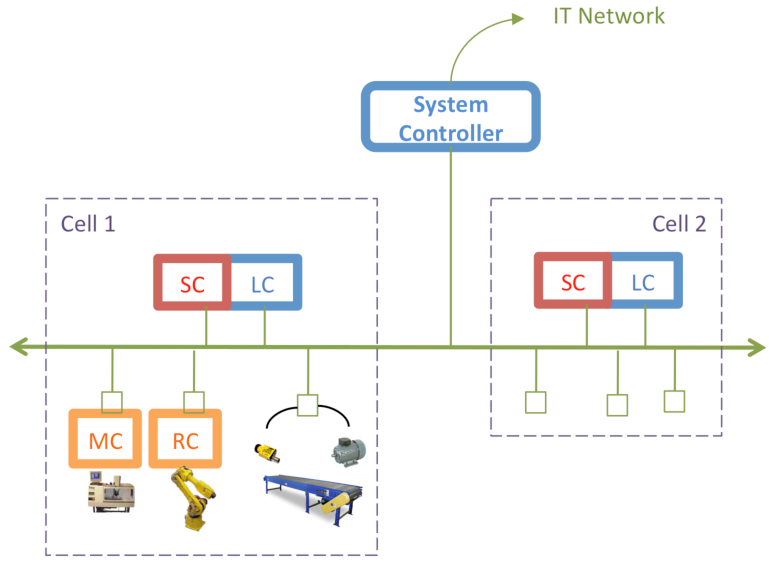
\includegraphics[width=0.95\columnwidth]{Figures/mfg-today.pdf}
\vspace{-\baselineskip}
\caption{Tomorrow's Manufacturing Control Systems.}%
\label{fig::today}
% \noindent \hrule
\vspace{-\baselineskip}
%\end{wrapfigure}
\end{figure}

% Move these over
\newcommand{\dst}{\mathcal{H}}

\section{\mfname Modeling Framework}
\subsection{Semantic Underpinnings}
We will use variables to model different state components of the plant and the controller. Each variable $v$ has an associated type denoted by $type(v)$ that is the set of values that $x$ can take.
Let $X$ be a set of variables. 
%
A {\em valuation\/} for $X$ is a function that maps each variable name $v \in X$ to a value in $type(v)$. The set of all possible valuations of $X$ is denoted by $val(X)$. 
Given a valuation  $x \in val(X)$, its restriction to a set of variables, $S \subseteq X$, is denoted by $x.S$. 
%(or states) of a set of variables $X$ is denoted by $val(X)$.

The overall system with a plant and a controller will be modeled as a \emph{discrete transition system\/}.
Formally, a transition system $\dst$  is a tuple $\langle X, \Theta, A, D \rangle$ where 
\begin{enumerate*}[label=(\roman*)]
	\item $X$ is a finite set of variables partitioned into $X= X_c \cup X_p$ sets of controller and plant variables; the set $val(X)$ of valuations of $X$ is called the set of {\em states.} 
    \item $\Theta \subseteq val(X)$ is a set of initial states, 
    \item $A$ is a finite set of actions partitioned into $A = A_c \cup A_p$ disjoint sets of controller and plant actions, and
    \item $D \subseteq val(X) \times A \times val(X)$ is the set of discrete state transitions. An individual transition  $(x, a, x') \in D$ is written as $x \arrow{a} x'$.
\end{enumerate*}
For a given state $x \in val(X)$, $x.X_p$ and $x.X_c$ are said to be the  plant and controller state at $x$.  
%
The plant variables ($X_P$) are read/write variables for the plant actions ($A_p$) and are only read by the controller actions ($A_c$).
That is, for any $x\arrow{a}x'$ with $a \in A_p$, $x.X_c = x'.X_c$.  
%
Similarly, the controller variables ($X_c$) are 
read/write variables for the controller actions ($A_c$) and are only read by the plant  actions ($A_p$).

An \emph{execution} of  $\dst$ is an sequence of states and transitions with plant and controller transitions alternating: $\alpha = x_0, a_1, x_1, a_2, x_2 \cdots$, where $x_0 \in \Theta$ and  $a_i \in A_c$  for  each odd $i$ and $a_i \in A_p$ for each even $i$ in the sequence.
A state $x$ is {\em reachable} if every there exists an execution that ends in $x$. 
Any set $I \subseteq val(X)$ that contains all the reachable states of $\dst$ is called an {\em invariant\/}. 
Invariants capture properties that must {\em always} hold for the system and can be stated in terms of plant and controller variables. 



\subsection{\mfname Modeling Overview}
\label{sec:model}

A \mfname model is specified by a the following three components: 
\begin{enumerate*}[label=(\roman*)]
	\item a plant that has a collection of cells where each cell can perform certain operations;
	\item  a set of widgets that move  through the cells and each widget is associated with a requirement that defines the sequence of operations that need to be performed on the widget for it to be complete; and
	\item a controller that orchestrates  the operations at cells and movement of widgets.
\end{enumerate*}
Next we formally describe each of these parts and in Section~\ref{sec:dts_def} we define the transition system model of the entire system that is defined by these three components.

 	
\subsection{Plant Description}
The plant models the floor plan of the factory, the layout of cells and the connections between them. There is a set $\OP$ of operations and the plant model specifies what cell can perform which of these operations on widgets. 
In addition, there are two special operation corresponding to creation ($\optop$) and removal ($\opbot$) of widgets. 
We define $\OPALL = \OP \cup \{\optop,\opbot\}$.


Formally, a  {\em plant\/} is specified by a tuple $P $ $=$ $\langle G_P, \Lmap_P{}, \Tmap_P{}, \Qmap_P{} \rangle$, 
    where 
    \begin{enumerate*}[label=(\roman*)]
      \item $G_P = \langle V_P,E_P \rangle$  is a graph of cells, where $V_P$ is the set of cells; the set of edges $E_P$ define the paths for moving widgets in the floor; 
%      \item $\OP$ is a set of (possible) operations;  
      \item $\Lmap_P{}: V_P \mapsto 2^{\OPALL}$ maps each cell to the set  of operations that can be performed at that cell;
      \item $\Tmap{}: V_P \times \OPALL \mapsto \mathbb{N}$ maps a cell $v \in V$ and an operation $op \in \Lmap(v)$ to a natural number $\Tmap{(v,op)}$ which is the amount of time (measured in number of transitions) needed to complete $op$ at $v$; 
      \item $\Qmap{}: V_P \mapsto \mathbb{N}$ maps each cell to its queue length $\Qmap{(v)}$, which is the maximum number of widgets that can be queued at $v$.
    \end{enumerate*}
For any graph and $G_P$ in particular, for any vertex $v \in V_P$
 $\next(v)$ and $\prev(v)$ denote the set of predecessors and successors of $v$ in $G_P$. 
 
\paragraph*{Sources and Sinks}
 A {\em source \/} is a cell $v \in V$ such that $\optop \in \Lmap{(v)}$ and $\prev(v) = \emptyset$.
A  {\em sink\/} is a cell $v$ with $\opbot \in \Lmap{(v)}$ and $\next(v) = \emptyset$.  
 For simplicity, in this paper we assume that there is a single source ($\verttop$) and a single sink ($\vertbot$)  in any plant $P$ and 
 that $ \Lmap{(\verttop)} = \{\optop\}$ and $\Lmap{(\vertbot)} = \{\opbot\}$. 
A cell in $V$ that is neither a source nor a sink is an {\em ordinary\/} cell. 

%\cy{CY: Should we mention that $\Tmap{v,op}$ is infinite (or zero?) if $op$ is not in $L_v$? (This is for some widgets to bypass a cell.)}
%\sayan{Yes, we may need this.}
	

\subsection{Widgets and Requirements}
For modeling convenience, we assume that there exists a universal set  $W$ of unique identifiers for {\em all} widgets that will ever be seen by the manufacturing system.
% 
This includes the actual widgets in the system, those that have been finished and those that are yet to start. We denote by $\Wtop$ the set of widgets that have not been created, that is, $W_\top = \{w \in W \ | \ \loc(w) = \verttop \}$. Similarly, $\Wbot$ is the set of widgets at the sink, and  $\Word = W \setminus (\Wtop \cup \Wbot)$.
For all the results presented in the paper, a sliding window of unique identifiers would be adequate. 
A possible implementation of this will be by attaching a unique RFID tag for each widget \cite{huang2008rfid}. 

A \emph{requirement models} the sequence of operations in $\OP$ that need to be performed on each widget for the widget to be completed. Formally, a requirement is specified by a directed acyclic graph (DAG) $R = \langle V_R, E_R \rangle$ and a labeling function $L_R:V_R\rightarrow {\OPALL}$.  Further, we require that there is a single vertex $v\ \in V_R$ with no incoming edges; this vertex is called the source of $R$ and $L_R(v) = \optop$. Finally, vertices with  no outgoing edges are called sinks, and every such vertex $v$ has $L_R(v) = \opbot$.
A {\em path\/} of $R$ is a sequence of vertices in $V_R$, $\pi = v_0,\ldots,v_k$ such that $v_0$ is the source, $v_k$ is a sink, and $(v_i,v_{i+1})\in E_R$ for each $i$ in the sequence. Given a path $\pi$, we define $L_R(\pi) =  L_R(v_0),\ldots,L_R(v_k)$ which is the corresponding sequence of operations in ${\OPALL}$.


\begin{example}
\label{ex:simple_plant}
%\sayan{Show a simple layout in figure. Define the corresponding graph and parameters also in Figure. This will be a running example throughout this section of the paper.}
Consider a manufacturing system consisting of three cells $V=\{v_1, v_2, v_3\} \cup \{\verttop, \vertbot\}$.
The plant can be represented as a graph $G=(V,E)$ shown as the graph below.
The circles in the graph are cells while black squares represent conveyors.
Then the operations that supported by a cell $v$ can be obtained by $L(v)$. For example, $L(v_3)=\{op_2,op_3\}$.
Let's further consider two widget types being fabricated in this plant.
Assuming requirement 1 requires to complete $op_1$ and $op_2$ and requirement 2 requires to complete $op_1$ and $op_3$ in the given order, then the requirements are denoted by $R_1=\{op_1 \ra op_2\}$ and $R_2=\{op_1 \ra op_3\}$, $\mathcal{R}=\{R_1, R_2\}$.

\begin{figure}[ht]
	\begin{center}
		\resizebox{0.3\textwidth}{!}{%
		    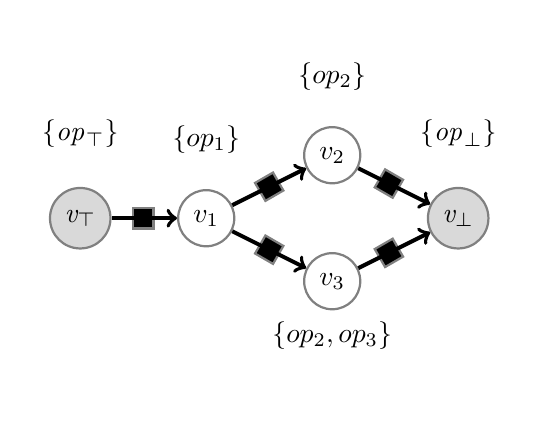
\begin{tikzpicture}
	    		%[scale=.8,auto=left,every node/.style={circle,fill=blue!20}]
	            [scale=0.8,auto=left,every node/.style={circle,draw=black!50, thick}, every path/.style={line width=0.5mm}]
	            
				\node[circle, fill=gray!30, label={$\{\optop\}$}] (v_o) at (-3,0) {$\verttop$};
	            \node[label={$\{op_1\}$}] (v_1) at (-1,0) {$v_1$};
				\node[label={$\{op_2\}$}] (v_2) at (1,1) {$v_2$};
				\node[label={[xshift=0cm, yshift=-2cm]\{$op_2,op_3\}$}] (v_3) at (1,-1) {$v_3$};
				\node[circle, fill=gray!30, label={$\{\opbot\}$}] (v_u) at (3,0) {$\vertbot$};
				
				\node[rectangle, fill=black, minimum size=7.5pt] (c_1) at (-2, 0) {};
				\node[rectangle, fill=black, minimum size=7.5pt, rotate=30] (c_2) at (0, 0.5) {};
				\node[rectangle, fill=black, minimum size=7.5pt, rotate=60] (c_3) at (0, -0.5) {};
				\node[rectangle, fill=black, minimum size=7.5pt, rotate=60] (c_4) at (1.9, 0.55) {};
				\node[rectangle, fill=black, minimum size=7.5pt, rotate=30] (c_5) at (1.9, -0.55) {};
				
				\path (v_o) edge[->] (v_1);
				\path (v_1) edge[->] (v_2);
				\path (v_1) edge[->] (v_3);
				\path (v_2) edge[->] (v_u);
	            \path (v_3) edge[->] (v_u);
		   \end{tikzpicture}
		}
	\end{center}
    \vspace{-0.25cm}
	\caption{The plant graph of a simple example.}
	\label{fig:exmaple_graph}
\end{figure}

\end{example}

\subsection{Concepts related to plants and requirements}
% Presenting these as concepts and later we say who computes what.
%In this section, we present several definitions that will be used throughout this paper.
%\sayan{Skipping this section for now. Feasible graphs/paths will probably come after introduction of controller.}
 
%Given a requirement $R = \langle O_R, E_R \rangle$ a $\mi{feasible graph}$ of a requirement $R$ is a subgraph of $G_P$ such that all paths in the $F_r$ satisfy all the paths in $R$. For a path in $F_r$ to satisfy a path in $R$, all the operations along a path in $R$ must be able to be completed by the cells along a path in $F_r$ in the same order. Note that this does not preclude a path from $F_r$ having cells which don't correspond to any node in $R$.

%Formally, a $\mi{feasible graph}, F_r = \langle V_r, E_r \rangle$ is a subgraph of $G_p$ where $V_r, E_r$ are subsets of $V_p, E_r$ respectively, Each path in $F_r$ begins at a $\mi{source}$ of the plant and terminates at a $\mi{sink}$. 
    
%\subsection{Additional Notation}
%This is a list of notation used in the plant/controller variables/transitions along with their explanations.
% Tree/Node operations
 
% Queue operations
Each $\queue(v)$ has the following operations: $\head$, returns the element at the front of the queue; $\len$, provides the current length of the queue up to a maximum specified by $\Qmap(v)$; and $\pop$, removes and returns the element at the head of the queue and decrements the $\len$ by one. 
% Additional notation
Additionally, we define the following notation: $\bag(v) := \{ w \mid \loc(w) = v\}$; $\Bag := \cup_{v \in V } \bag(v)$.

\subsection{Discrete Transition System}
\label{sec:dts_def}
We now describe the nominal  plant and an abstract controller. 
Additional variables may be added to this model, for example, to implement specific  controllers strategies and to track more complex performance metrics. 

\subsubsection*{Plant Variables}
\figref{plant-variables} gives the names and types of the plant variables ($X_p$).
The  variable $\loc$ gives the  cell at which each widget is located. Initially, all widgets are at the source $\verttop$, which indicates that they have not yet been created. When a widget is consumed at a sink its location is set to $\vertbot$. 
%
The plant variable $\pos$ assigns, for each widget, $w \in \Word$ a natural number. If $\loc(w) \in V$ then $\pos \leq Q(loc(w))$ and it is the actual position of $w$ in the queue of $\loc(w)$ (otherwise, $w \notin \Word$ and $\pos(w)$ is meaningless).
%
The variable $\queue$ is the queue (array) of widgets at that cell. As specified by the plant $P$, for any cell $v \in V_P$, the length of $\queue(v)$ is upper bounded by $Q(v)$. Initially, the queue is empty (\ie all entries are set to $\bot$).
%
The variable $\req$ selects and assigns a requirement $R \in \mathcal{R}$ to a widget. The selection of $R$ will determine the set of operations that are performed on the widget. 
%
Finally, $\widgettime$ tracks the total time a widget spent in the plant starting from $\verttop$ and ending at $\vertbot$. All widgets have their $\widgettime$ initialized to 0.

\begin{figure}[!ht]
	\centering
	\mybox{\linewidth}{\linewidth}{
		\lstinputlisting[language=ioaNums,numbersep=-3pt]{Specifications/plant_vars.txt}
		\caption{\scriptsize Plant ($X_p$) variables and types.}
	\figlabel{plant-variables}
	}
\end{figure}

\subsubsection*{Abstract Controller Variables}
\figref{abstract-cell-variables} shows the list of abstract controller variables:
%The controller variable $\completed$ keeps track of the sequence of operations that have been performed on each widget. Initially, it is the empty sequence for every widget. 
The $\timer$ keeps track of the current time of the  overall system.
%
The variable $\action$ encodes the actuation decision made by the controller for each cell $v$ for the following plant transition in which the cell $v$ uses the decision to perform some operation.
%
The variable $\nexttr$ specifies for each cell $v$ a neighboring cell   to which $v$ should transfer a widget  when it receives a  $\transfer$ action controller.
%
A concrete controller uses these and other variables to make decisions and keep track of the overall system state. 

\begin{figure}[!ht]
	\centering
	\mybox{\linewidth}{\linewidth}{
		\lstinputlisting[language=ioaNums,numbersep=-3pt]{Specifications/abstract_cell_vars.txt}
		\caption{\scriptsize Abstract controller variables.}
	\figlabel{abstract-cell-variables}
	}
\end{figure}

\subsubsection*{Plant Transitions}
During each plant transition, all the cells are updated  based on the decisions made by the controller that are reflected in the controller variables such as $\action$. These variables are read by the plant.
An ordinary operation $\op \in OP$ causes the plant to perform this operation on the current widget. There are several special actions: $\move$  moves widgets on conveyors, $\optop$ creates new widgets at sources, $\opbot$ removes finished widgets at sinks and $\transfer$ moves widgets between adjacent connected cells in the plant. We now discuss these transitions in more detail.

% Move action
If a conveyor cell $v$ is provided with a $\move$ action, $v$ decrements the position of each of the widgets in $\queue(v)$.
% OP action
If a cell is given the $\OP$ action, the cell starts to perform $\op$ on the widget at the head of its queue. While this presumably changes the local physical state of the plant and the widget, in our model, this action does not change any plant variables. Instead, we will see later that once $\op$ completes then the controller will update the record for the widget. 

% Instantiate action
If a source cell $v$ is given the $\optop$ action, it selects a widget from $w' \in \Wtop = \bag(\verttop)$, the set of widgets at the source,  $\verttop$, and assigns it a requirement $R$. This nondeterministic choice models the uncertainty in the type of requirement that is demanded from the next widget. The location of the new widget $w'$ is set to be $\verttop$ and its position is set to the end of its queue.
%
% Terminate action
If a sink cell is given the $\opbot$ action, the cell will remove the widget from the head of its queue and the removed widget's location is set to  $\vertbot$.
%
% Noop action
If a cell is given a $\noop$ action, the cell does not change any of the variables.
%
% Transfer action
If a cell is given a $\transfer$ action, the cell removes the widget at the head of its queue and reads the $\nexttr$ variable to determine the next cell to transfer the removed widget. The cell transfer the widget to the next cell by changing the location of the widget to that of the next cell and the position to the end of the next cell.


% THIS IS FOR THE ABSTRACT CONTROLLER
%\subsection*{Controller Transitions}
%During each controller transition, the controller increments $\timer$ by 1 and iterates through all the cells to update their $\cost$, $\action$, and $\nexttr$ variables.

\begin{figure}[!ht]
	\centering
	\mybox{\linewidth}{\linewidth}{
		\lstinputlisting[language=ioaNums,numbersep=-3pt]{Specifications/plant_trans.txt}
		\hfill
		\caption{\scriptsize Plant ($X_p$) transitions.}
        \figlabel{plant-transitions}
        }
\end{figure}



\section{Baseline Controller}
\label{sec:baseline-controller}

In this section, we present a basic centralized controller strategy which is a refinement of the abstract controller of \figref{abstract-cell-variables}. Controllers make the following decisions:  (a) plan a sequence of operations according to the requirements of a widget, (b) map these operations on to appropriate cells, and (c) orchestrate the movement and operation of the widgets and cells. In presenting the controller, we first introduce the formal notion of a {\em plan} that encapsulates the first two pieces. 

\subsection{Plans and Feasible Graphs}
Recall, given a requirement $R$ and a plant $P$,  $G_P =\langle V_P, E_P \rangle$ is the graph of cells for the plant and
 $G_R = \langle V_R, E_R \rangle$ is the graph of the requirement. A {\em plan} $\plan$ is essentially a forward simulation relation from $V_R$ to $V_P$~\cite{lyn:fbs}. That is, it is a relation $\plan \subseteq V_R \times V_P$ such that for any $(v_{1R},v_{1P}) \in \plan$ and  $(v_{1R},v_{2R}) \in E_R$, there is {\em a path\/}  $\pi = v_{1P}, \ldots, v_{2P}$ in the plant graph, such that 
(a) $(v_{2R},v_{2P}) \in \plan$, and  
(b) $L_R(v_{2R}) \in L_P(v_{2P})$.
 %
 In other words, a plan relates vertices in $V_R$ to vertices in $V_P$ so that each edge $(v_{1R},v_{2R})$ in the requirement graph can be simulated by paths $G_P$ and the first and the last vertices in the path are at cells that can perform the operations required at  $(v_{1R},v_{2R})$.
 %
 
 The above definition of plan allows each operation in the requirement $R$ to be accomplished by traversing an arbitrary but finite path (i.e., sequence of cells) in $G_P$. A path corresponding to a single edge in $E_R$ may revisit the same cell in $G_P$ multiple times. 
%This is in stark contrast with routing works in SDNs. 
 %
We can show this using a standard simulation argument~\cite{lyn:fbs}. Therefore, a plan gives a set of feasible paths for achieving the requirement $R$ in the plant $P$. 
 \begin{proposition}
 	\label{prop:paths}
 	There exists a plan for a requirement $R$ and plant $P$ if and only if for every path of $G_R$ there exists a corresponding path in $G_P$.	
 \end{proposition}
 
 
 In order to obtain performance guarantees, concrete controllers will restrict the family of paths. For example, for every edge in $(v_{1R},v_{2R}) \in E_R$, the corresponding path $\pi = v_{1P}, \ldots, v_{kP}$ in $G_R$ may be required to satisfy one of these conditions:
%
 \begin{itemize}
 	\item 	{\em $k$-cell repetitions\/}:  each cell $v \in G_P$ may repeat in $\pi$ at most $k$ times. For $k=1$ this implies that a cell may be visited at most once including at $v_{2P}$. 
 	% 
 	\item {\em $k$-op misses\/}: the number of cells $v$ such that $L_R(v_{2R}) \in \Lmap_P(v)$ in the path is at most $k$. For $k=1$ this implies that there is only one cell $v_{2P}$ in $\pi$ with $\Lmap_R(v_{2R}) \in \Lmap_G(v_{2P})$ is where the operation $\Lmap_R(v_{2R})$ is performed. 
 	\end{itemize}
% 
Given a $\plan$ and path $\pi$ in $G_R$, the corresponding set of paths in $G_P$ constructed from $\plan$ are called the {\em feasible paths} of $\pi$.  The set of all the feasible paths corresponding to $R$ in $G_P$ is called the {\em feasible graph\/} and is denoted by $F_{R,P}$. 
We now proceed to describe our baseline controller that constructs and uses a particular class of plans
represented as feasible graphs. 
 
 
\subsection{Implementation of Baseline Controller}

\subsubsection*{Controller Variables}
\figref{controller-variables} gives the names and types of our controller variables ($X_p$).
Any variables that overlap with the abstract controller variables take on the same definition as  before unless explicitly stated otherwise.
% Action variable
%The variable $\action$ encodes the actuation decision made by the controller for each cell for the following plant transition in which the cell uses the decision to perform some operation.
% Completed variable
The controller variable $\completed$ keeps track of the sequence of operations that have been performed on each widget. Initially, it is the empty sequence for every widget. 

The $\ptr$ variable of a widget is a pointer into Plan  corresponding to the same requirement as that of the widget. This variable keeps track of what operation should currently be performed on a widget at a particular cell and which path through the plant to take.
% Starttime variable
The variable $\starttime$ marks the start of a new operation by a cell and is used track how long a particular operation has been ongoing. 
%
The $\waittime$ variable monitors the amount of time a cell has been waiting for the $\transfer$ action to move a widget from the head of its queue.

% Pointer variable
% Status variable
A cell's $\status$ denotes the current condition of the plant and can be one of the three following states: $\idle$, the cell is not working on any widget; $\operational$, the cell is performing some $\op \in \OP$ on a widget at the head of the cell's queue; and $\waiting$, the cell has completed $\op \in \OP$ and the cell is waiting for a $\transfer$ action to move the widget at the head of its queue further along in the plant.
% Timer variable
%The $\timer$ tracks the total time that has passed since the start of the simulation. It is incremented at the start of every controller transition update.
% Waittime variable
% Cost variable
The $\cost$ variable maps a cell's state to a real number which can be used to choose between feasible paths in order to optimize with respect to a cost metric (for example, energy, reliability, etc.). 

%This weight is used in computing an optimal path that a widget will follow through the plant. The optimality of the path is dependent on the types of metrics one is trying to optimize for.

\begin{figure}[!ht]
	\centering
	\mybox{\linewidth}{\linewidth}{
		\lstinputlisting[language=ioaNums,numbersep=-3pt]{Specifications/cell_vars.txt}
		\hfill
		\caption{\scriptsize Controller ($X_c$) variables and types.}
	\figlabel{controller-variables}		
	}
\end{figure}

\subsubsection*{Controller Transitions}
During each controller transition, the controller first increments $\timer$ by 1 and performs the following three major steps: 
\begin{enumerate*}[label=(\roman*)]
    \item determines the shortest path in each feasible graph $F_{R,G}$ according to the chosen cost metric; 
    \item updates each of the $\nexttr$ and $\action$ variables for each cell; and
     \item possibly updates the $\cost$ of each cell in the plant.
\end{enumerate*}
We discuss these steps in some more detail.
From the statically computed feasible graphs $F_{R,P}$, the controller runs a shortest path algorithm utilizing the recently set costs to determine the best paths through the plant.
The controller iterates through each $v \in V$ and first sets the $\nexttr$ variable to the the cell with the lowest cost from the set $\next(v)$. Next, the controller determines the action that the cell should take depending on its type. If the $\celltype(v)$ is a conveyor cell, a $\move$ action is done unless there is a widget at the head of the queue; otherwise, the cell increments its $\waittime$ by 1. If the type is a source cell, the controller checks whether a widget already exists in the cell's queue. If so, then the controller tries to transfer the widget to the next cell, otherwise, it instantiates a new widget. If type is an ordinary cell, the controller cycles between the $\idle$, $\operational$, and $\waiting$ states to determine the correct action. If the cell's status is $\idle$, the controller either tries to transfer the widget immediately in the case of a $\noop$ operation or performs an $\op$ action if there is a widget at the head of the queue; otherwise, the cell does nothing. If the cell's status is $\operational$, the controller assigns the action $\op$ to the cell until the $\op$ has been completed at which point the controller sets the cell's status to waiting. If the cell's status is $\waiting$, the controller tries to transfer the widget. If the transfer is successful, the controller changes the cells's status to $\idle$ and the cycle repeats. Additionally, regardless of state, if the cell has space on its queue, it will try to enqueue a widget from one of its input conveyors with the largest $\waittime$ one of its input conveyors, specifically the input conveyor with the largest waiting time. If the type is a sink cell, the controller instructs the cell to either terminate a widget at $\head(\queue(v)))$ or do nothing.
%\end{enumerate}

\begin{figure}[!ht]
	\centering
	\mybox{\linewidth}{\linewidth}{
		\lstinputlisting[language=ioaNums,numbersep=-3pt]{Specifications/cell_trans.txt}
		\hfill
		\caption{\scriptsize Controller ($X_c$) transitions.}
        \figlabel{controller-transitions}
	}
\end{figure}
\subsection{Rigorous Reasoning about Properties}
\label{sec:prop}
Our \mfname framework is designed to support rigorous analysis of correctness and performance properties of the system. The formal framework will support standard reasoning in terms of invariants, abstractions,  substitutivity and will be eventually supported by  computer-aided verification tools~\cite{IOA89}.
%
While a full verification of our baseline controller is beyond the scope of the current paper, we present several key assertions and arguments to sketch the outline of a correctness argument. Additionally, the baseline controller we present here uses a subset of the global view available to it and makes decisions based on a local level. Much more complex controllers can be implemented with \mfname such as those presented in literature~\cite{Taylor2015}.

The following invariant  captures the mutual exclusion property and ensures that there is no ``pile-up'' of widgets on cell and conveyors. 
\begin{proposition}
\label{prop:mutex}
 For any ordinary cell $v \in V_P\setminus \{\verttop,\vertbot\}$, and any two distinct widgets $w_1, w_2 \in W$,
 if $w_1, w_2 \in \bag(v)$ then $\pos(w_1) \neq \pos(w_2)$.
 \end{proposition}	
This invariant is  proved by induction on  the length of any execution of the $\dst$. 
The base case (an execution of length $0$) holds vacuously, because at any  initial state of $\dst$, all the widgets are at the source $\verttop$. For the inductive step, we check for each possible plant and controller transition to verify that the invariant is preserved. This involves a case analysis across all the {\bf if\/} conditions in \figref{plant-transitions} and \figref{controller-transitions}. The $\canenqueue$ variable restricts the $\transfer$ action from occurring unless there is an empty space at the end of the queue for any cell.

The following invariant  captures the correctness property that ensures that only complete widgets appear at the sink.
\begin{proposition}
	\label{prop:completeness}
	For any sink $\vertbot$, and any widget $w \in \bag(\vertbot)$, the widget is completed, i.e., 
	$\completed(v)$ is a path in $\req(w)$. 
\end{proposition}
This invariant is derived from a stronger invariant that captures the relationship between the $\completed(v)$ variable and the position of the widget and the feasible graph. 
Roughly, a widget $w$ with requirement $R$ follows a path in the plant following only the nodes of a feasible graph $F_{R,P}$. From Proposition~\ref{prop:paths} it follows that, as $w$  traverses the plant from a source $\verttop$ to a sink $\vertbot$ it must follows a path in $G_R$, and therefore, when it appears at $\vertbot$ it is complete. 

The next proposition  captures the  property that all widgets complete within bounded time for any plant that is a directed acyclic graph (DAG). 
\begin{proposition}
	\label{prop:timebound}
For any acyclic requirement and any widget $w\in V_o$, there exists a $k>0$ such that if $\widgettime(w) \geq k$ then $w \in \bag(\vertbot)$.
\end{proposition}
%All widget must go through the system in finite time
Since $G_P$ has finite depth in this case, the property is established by  showing that $w$ traverses an edge from $loc(w)$ in the plant graph $G_P$ in finite time. 
%
For plants with cycles, this property may not hold with our baseline controller as widgets may deadlock.
%Sketch of proof: This will depend on how the controller tells cells to enqueue their widgets unto the next cell. I am considering the notion of first come, first serve. Suppose that there are two conveyors, $c1, c2$ that feed into a single machine and that at time $t$, both conveyors get a widget in the head of the queue. Whenever a widget is pushed to the head, it is assigned a $waiting\_time$ of how long it has been waiting in the head to be enqueued. The controller will select to enqueue the widget from the conveyor whose waiting time is greater. In the case of ties, the controller, can randomly select the widget to be enqueued.

%List of properties that the controller should satisfy and ideas for how to prove these
%\begin{enumerate}
%	\item Given a widget assigned requirement $R$, after the widget has passed through the plant from the source to the sink, the list of its completed operations should match one of the paths of the widget's corresponding requirement.
%    
%    Sketch of proof: The proof will make use of FeasibleGraphs. Each path in the feasible graph is a path through the plant that satisfies all the operations and their orderings as specified by requirement $R$. Feasible Graphs are computed by using a graph matching algorithm. 
    
%    \item  
%\end{enumerate}


%\subsection{Formal}
%Formally defining the properties:
%\begin{enumerate}
%	\item Correctness: $\forall v \in \bag(\vertbot) \Rightarrow \completed(v) \in \req(v)$ 
%    The list of operations completed by all widgets in the completed pool should satisfy their corresponding requirement. 
%    
%    
%    \item Completeness: $\forall w \in \bag(\verttop) \Rightarrow \widgettime(w) \leq T_R$
%    For each completed widget, the total time it took to travel through the plant should be bounded by some time $T_R$.
%    
%   
%\end{enumerate}


\input{Sections/approach}
\section{Modeling a Realistic Manufacturing Testbed}
\label{sec:smart}

To  demonstrate the expressive power of our modeling framework we present a formal model of the System-level Manufacturing and Automation Research Testbed (SMART), a realistic testbed at the University of Michigan.

\subsection{SMART System Overview}
\label{subsec:smart_overview}
SMART is a hybrid serial-parallel line manufacturing testbed at University of Michigan~\cite{ilya:smart} (see Figure~\ref{fig:smart_layout}). It has three cells and two conveyor lines connected with a controllable pneumatic diverter. There are three industrial robots and four CNC milling machines that can produce discrete products.

Blocks 1 and 2 each contain two CNC machines and a six degree of freedom robotic arm.
Each of the CNCs are controlled by a PLC and are pre-programmed to perform operations based on the inputs from central controller (in our model, the central controller is the baseline controller). The robotic arm is programmed to pick and place parts between the conveyor and the CNCs one at a time. Blocks 1 and 2 are linked with a single conveyor line. The conveyor from Block 2 branches out into two separated conveyors going to Blocks 1 and 3. There is a diverter at the conveyor fork that determines which branching conveyor a widget takes. Block 3 contains the last robotic arm in the system that is used for additive manufacturing.

The SMART system has various sensors for gathering plant and widget state information. A camera system captures images of the widgets. 
%The widgets are carried by pallets moving around on the testbed via the conveyor system.
There are RFID transceivers and seven proximity sensors installed for locating widgets.
Each widget is  labeled with a unique RFID tag and  ID. 
The RFID tags have re-write capabilities, which can be used to store operation data such as the $\completed{}$ variable. 
%All six RFID transceivers are able to read and write data for each tag.
%SMART collects all possible data flowing in the plant.
%Besides the working part information detected and read by the proximity sensors and RFID transceivers, operational data is also recorded.
For each CNC, the motor's position for each axis and the load on the motor are captured.
For each robotic arm, the position of the joints and end effector are obtained from the robot controller.
Energy consumption of SMART is also measured and recorded for the conveyors, robotic arms and one of the CNCs.  
The collected data is sent to the central controller.
% configure PLC logic.


\begin{figure}[t]
%\vspace{-\baselineskip}
\centering
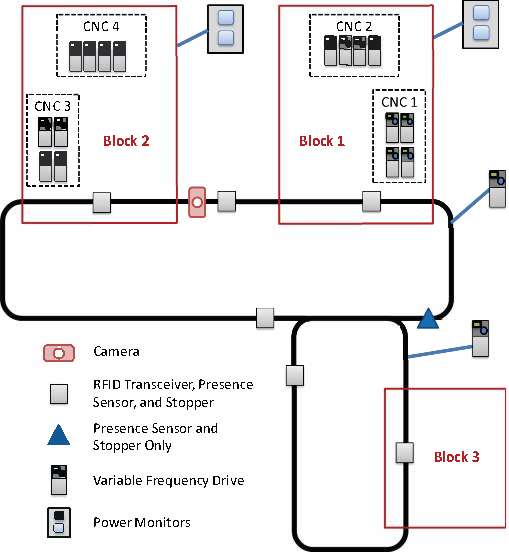
\includegraphics[width=0.7\columnwidth]{Figures/SMART_layout}
%\vspace{-\baselineskip}
\caption{\small Layout of the SMART testbed.}
\label{fig:smart_layout}
%\vspace{-1\baselineskip}
\end{figure}

\begin{figure}[t]
%\vspace{-\baselineskip}
\centering
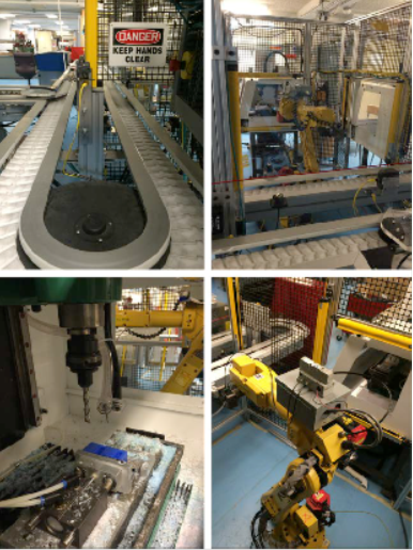
\includegraphics[width=0.6\columnwidth]{Figures/SMART_photos}
%\vspace{-\baselineskip}
\caption{\small Machine cells and conveyors.}
\label{fig:smart_photos}
%\vspace{-1\baselineskip}
\end{figure}



\begin{figure}[t]
	\begin{center}
		\resizebox{0.4\textwidth}{!}{%
		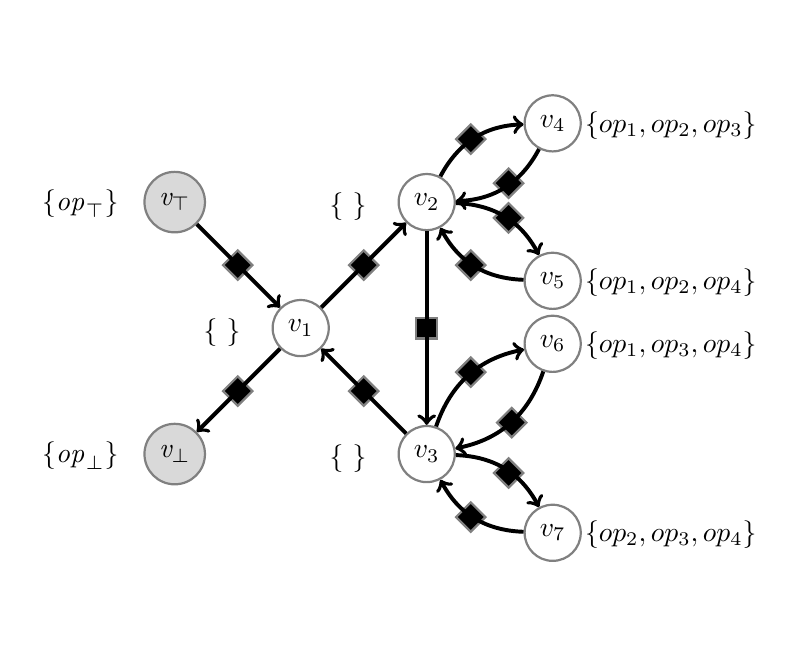
\begin{tikzpicture} 
			%[scale=.8,auto=left,every node/.style={circle,fill=blue!20}]
            [scale=.8,auto=left,every node/.style={circle,draw=black!50, thick},every path/.style={line width=0.5mm}]
            
%			\node[circle, fill=gray!30, label={[xshift=-1.2cm, yshift=-1.1cm, align=left]$\{\optop\}$\\test 2nd line}] (v_o) at (-3,2) {$\verttop$};
			\node[circle, fill=gray!30, label={[xshift=-1.2cm, yshift=-1.1cm, align=left]$\{\optop\}$}] (v_o) at (-3,2) {$\verttop$};
            \node[circle, fill=gray!30, label={[xshift=-1.2cm, yshift=-1.1cm]$\{\opbot\}$}] (v_u) at (-3,-2) {$\vertbot$};
            
            \node[label={[xshift=-1cm, yshift=-0.9cm]$\{\ \}$}] (v_1) at (-1,0) {$v_1$};
			\node[label={[xshift=-1cm, yshift=-0.9cm]$\{\ \}$}] (v_2) at (1,2) {$v_2$};
			\node[label={[xshift=-1cm, yshift=-0.9cm]$\{\ \}$}] (v_3) at (1,-2) {$v_3$};
            
            \node[label={[xshift=1.5cm, yshift=-1.65cm]$\{op_1,op_2,op_3\}$}] (v_4) at (3,3.25) {$v_4$};
            \node[label={[xshift=1.5cm, yshift=-1.65cm]$\{op_1,op_2,op_4\}$}] (v_5) at (3,0.75) {$v_5$};
            \node[label={[xshift=1.5cm, yshift=-1.65cm]$\{op_1,op_3,op_4\}$}] (v_6) at (3,-0.25) {$v_6$};
            \node[label={[xshift=1.5cm, yshift=-1.65cm]$\{op_2,op_3,op_4\}$}] (v_7) at (3,-3.25) {$v_7$};
			

		\node[rectangle,fill=black,minimum size=7.5pt,rotate=45] (v_c) at (-2,1) {};				\node[rectangle,fill=black,minimum size=7.5pt,rotate=45] (v_c) at (0,1) {};
		\node[rectangle,fill=black,minimum size=7.5pt,rotate=45] (v_c) at (-2,-1) {};				\node[rectangle,fill=black,minimum size=7.5pt,rotate=45] (v_c) at (0,-1) {};
		\node[rectangle,fill=black,minimum size=7.5pt] (v_c) at (1,0) {};
		
		\node[rectangle,fill=black,minimum size=7.5pt,rotate=45] (v_c) at (1.7,-0.7) {};	
		\node[rectangle,fill=black,minimum size=7.5pt,rotate=45] (v_c) at (1.7,1) {};
		\node[rectangle,fill=black,minimum size=7.5pt,rotate=45] (v_c) at (1.7,3) {};
		\node[rectangle,fill=black,minimum size=7.5pt,rotate=45] (v_c) at (1.7,-3) {};
		
		\node[rectangle,fill=black,minimum size=7.5pt,rotate=45] (v_c) at (2.3,2.3) {};
		\node[rectangle,fill=black,minimum size=7.5pt,rotate=45] (v_c) at (2.3,-2.3) {};
		
		\node[rectangle,fill=black,minimum size=7.5pt,rotate=45] (v_c) at (2.3,1.75) {};
		\node[rectangle,fill=black,minimum size=7.5pt,rotate=45] (v_c) at (2.35,-1.5) {};		
						
			\path (v_o) edge[->] (v_1);
            \path (v_1) edge[->] (v_u);
			\path (v_1) edge[->] (v_2);
			\path (v_2) edge[->] (v_3);
            \path (v_3) edge[->] (v_1);
            \path[]
            	(v_2) edge[<-,bend right] (v_4)
                (v_2) edge[->,bend left] (v_4);
            \path[]
            	(v_2) edge[<-,bend right] (v_5)
                (v_2) edge[->,bend left] (v_5);
			\path[]
            	(v_3) edge[<-,bend right] (v_6)
                (v_3) edge[->,bend left] (v_6);
            \path[]
            	(v_3) edge[<-,bend right] (v_7)
                (v_3) edge[->,bend left] (v_7);                
       
		\end{tikzpicture}
	}
	\end{center}
	\caption{\small The graph representation of SMART for the formal model.}
	\label{plantgraph}
\end{figure}


\subsection{Modeling SMART System}
\label{subsec:smart_setup}
%The case study is constructed based on SMART.
A discrete transition system model $\dst$ for SMART is obtained once we specify the  plant, a controller, and a requirement. We will use the baseline controller for this demonstration. 

In order to create the plant model for SMART, we consider Block 3 as the place where widgets enter and leave the plant (there are two product bins, one with raw parts and another with finished part).
The robotic arm in Block 3 picks a raw part from the corresponding product bin and places it on the conveyor to introduce a new part to the plant.
This corresponds to the creation of a new widget at a source node. 
A finished part has to reach Block 3 where the robotic arm picks the part from the conveyor and places it into the finish part's product bin. This sequence of actions corresponds to a part being consumed.
%
Since in our model source and sink vertices have to be distinct, we  use two separate vertices $\verttop$ and $\vertbot$  in the plant graph $G_P$ (see Figure~\ref{plantgraph}). 
In practice, this corresponds to logically splitting the Segment into two cells.
%start node and end node.
%
%creation of a new widget at a source node. 
%We assume there is no limit in space for the product bins.
%
Since all four CNCs can perform operations in parallel, we model each of the CNCs as a single cell in $G_P$.
There are four different operations $(\OP)$, listed in Table~\ref{tab:smart_operation_time}.
%We assume that parts are queued on the conveyors.
\begin{table}[!t]
\centering
\caption{\small Time $T_P$ for each CNC machine to complete operations.}
\label{tab:smart_operation_time}
\begin{tabular}{|c|c|c|c|c|}
\hline 
 & CNC 1 ($v_4$) & CNC 2 ($v_5$) & CNC 3 ($v_6$) & CNC 4 ($v_7$) \\ 
\hline \hline
$op_1$ & 20 & 25 & 35 & -- \\ 
\hline 
$op_2$ & 50 & 30 & -- & 10 \\ 
\hline 
$op_3$ & 25 & -- & 15 & 30 \\ 
\hline 
$op_4$ & -- & 10 & 25 & 30 \\ 
\hline 
\multicolumn{5}{l}{* all values are scaled to transition time ticks} \\
\multicolumn{5}{l}{* ``--'' indicates that the operation is not supported on this machine}
\end{tabular} 
\end{table}

\begin{table}[!t]
\centering
\caption{Operation requirements. Three requirements are considered in the case study in SMART.}
\label{tab:smart_requirements}
\begin{tabular}{|c|l|}
\hline
 & \multicolumn{1}{c|}{Operations}            \\ \hline \hline
$R_1$         & $\optop \ra op_1 \ra op_2 \ra op_3 \ra op_4 \ra \opbot$ \\ \hline
$R_2$         & $\optop \ra op_1 \ra op_3 \ra op_1 \ra \opbot$  \\ \hline
$R_3$         & $\optop \ra op_2 \ra (op_3\ , \ op_4) \ra op_1 \ra \opbot$  \\ \hline
\end{tabular}
\end{table}    

%\subsection{Formal Model}
%\cy{To be finished.}

The robot arms and the diverter act as forks in the plant that allow widgets travel along any of the forking paths. To capture this behavior, they are modeled as cells that only perform a $\noop$ operation.



Consider three types of widgets to be fabricated on SMART.
The requirement for each widget type is given in Table~\ref{tab:smart_requirements}.
The symbol ``--'' indicates that the operation is not supported by the corresponding CNC machine in that column.

Requirement 1 ($R_1$) is a typical manufacturing process that requires a sequence of different operations.
In this case, all four operations have to be performed in the given order for this type of widgets.
Requirement 2 ($R_2$) is a slightly different process. 
It is comprised of two types of operations but requires $op_1$ to be revisited in the end.
%This is common 
Requirement 3 ($R_3$) shows a more variant process.
The first operation in $R_3$ is mandatory.
 	
\section{\mfname Simulator}
\label{sec:simulation}

We have developed a flexible, open source, discrete event simulator capable of simulating arbitrary \mfname models. The simulator is developed in Python3 and uses the Graphviz and Matplotlib libraries to visualize all outputs. The simulator is available for download at \url{https://github.com/SDC-UIUC/synthesis}.

The \mfname simulator takes as input plant and requirement files specified in the YAML format. The plant input file specifies all the cells with the operations they support and their times and all the conveyors with their lengths and the cells they connect to. The requirement input file specifies all the various requirements one would like to run against the plant. Each requirement contains a list of nodes with a single operation and a list of edges to link these nodes. Examples of both types of input files can be found at the link above. 

During a single execution of the simulator, it first parses the user input and then create graphs of the inputs in the DOT language. Each graph is then written to a PNG file to allow users to visually verify that the simulator constructed the plant/requirement graphs correctly. Next, the simulator executes the system for a specified amount of time using the baseline controller (others can be coded). To make the system run deterministically, the sources assign requirements in a round-robin fashion to widgets whenever they are instantiated. At every time step, the simulator moves widgets around in the plant, updates the states of each cell and logs various metrics: throughput, end-to-end delay, and the number of live widgets in the plant at a given time. At the end of execution, the simulator will output a log file to show the state of every cell in the system and all live widgets at every time step. Additionally, it creates and saves the plots for all the metrics listed above.
\begin{figure}[b]
\begin{center}
	\resizebox{0.4\textwidth}{!}{%
 		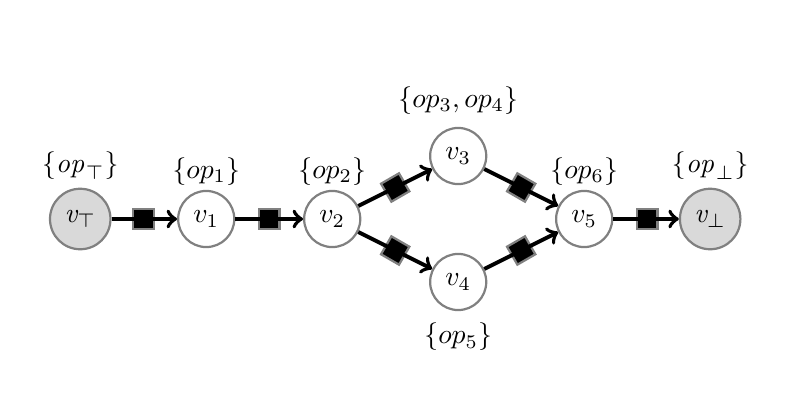
\begin{tikzpicture} 
 %[scale=.8,auto=left,every node/.style={circle,fill=blue!20}]
             [scale=.8,auto=left,every node/.style={circle,draw=black!50, thick},every path/.style={line width=0.5mm}]
 			\node[circle, fill=gray!30,label={[xshift=0cm, yshift=-0.4cm]$\{\optop\}$}] (v_t) at (-5,0) {$\verttop$};
             \node[label={[xshift=0cm, yshift=-0.4cm]$\{op_1\}$}] (v_1) at (-3,0) {$v_1$};
             \node[label={[xshift=0cm, yshift=-0.4cm]$\{op_2\}$}] (v_2) at (-1,0) {$v_2$};
             \node[label={[xshift=0cm, yshift=-0.6cm]$\{op_3,op_4\}$}] (v_3) at (1,1) {$v_3$};
             \node[label={[xshift=0cm, yshift=-1.7cm]$\{op_5\}$}] (v_4) at (1,-1) {$v_4$};
             \node[label={[xshift=0cm, yshift=-0.4cm]$\{op_6\}$}] (v_5) at (3,0) {$v_5$};                         
 			\node[circle, fill=gray!30,label={[xshift=0cm, yshift=-0.4cm]$\{\opbot\}$}] (v_b) at (5,0) {$\vertbot$};
			
			\node[rectangle,fill=black,minimum size=7.5pt] (v_c) at (-4,0) {};			
			\node[rectangle,fill=black,minimum size=7.5pt] (v_c) at (-2,0) {};
			\node[rectangle,fill=black,minimum size=7.5pt,rotate=30] (v_c) at (0,0.5) {};             
			\node[rectangle,fill=black,minimum size=7.5pt,rotate=60] (v_c) at (0,-0.5) {};          
			\node[rectangle,fill=black,minimum size=7.5pt,rotate=60] (v_c) at (2,0.5) {};  
			\node[rectangle,fill=black,minimum size=7.5pt,rotate=30] (v_c) at (2,-0.5) {}; 
			\node[rectangle,fill=black,minimum size=7.5pt] (v_c) at (4,0) {}; 	
			\node[rectangle,fill=black,minimum size=7.5pt] (v_c) at (-2,0) {};  		
			
 			\path[line width=0.5mm] (v_t) edge[->] (v_1);
 			\path (v_1) edge[->] (v_2);
 			\path (v_2) edge[->] (v_3);
 			\path (v_2) edge[->] (v_4); 
 			\path (v_3) edge[->] (v_5); 						
 			\path (v_4) edge[->] (v_5);
 			\path (v_5) edge[->] (v_b);
 		\end{tikzpicture}
 	}
 	\end{center}
\caption{The plant graph of the linear model case.}
\label{fig:linear_plant_graph}
\end{figure}


\begin{figure*}[!t]
\centering
    \begin{subfigure}[t]{0.33\linewidth}
        \centering
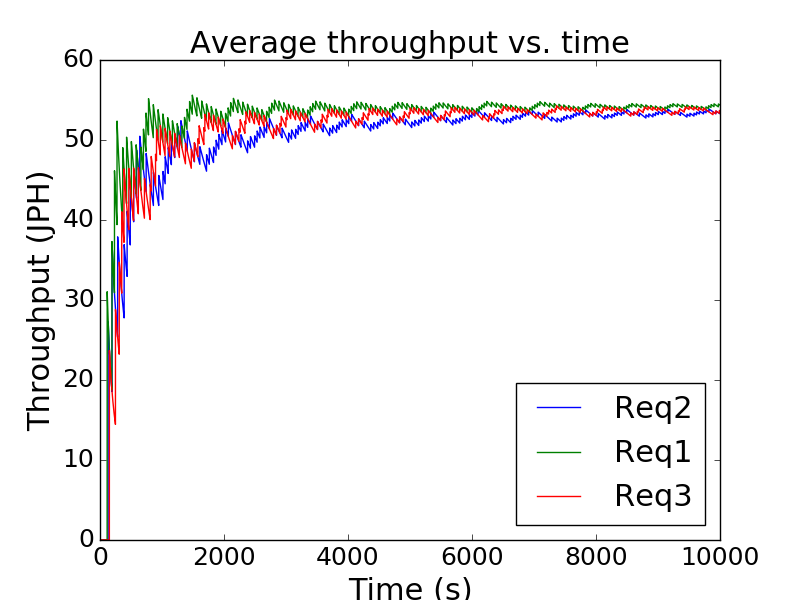
\includegraphics[width=0.99\columnwidth]{Figures/b2-throughput}
%\vspace{-\baselineskip}
\caption{Throughput of each widget (JPH).}
\label{fig:linear_jph}
%\vspace{-1\baselineskip}
    \end{subfigure}%
        ~%\hspace{0.5cm} 
    \begin{subfigure}[t]{0.33\linewidth}
        \centering     
        %\vspace{3\baselineskip}     
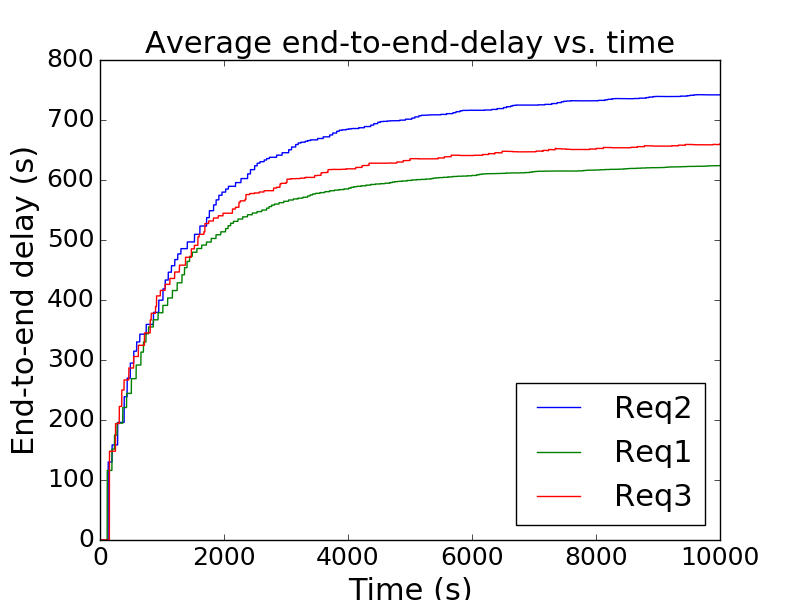
\includegraphics[width=0.99\columnwidth]{Figures/b2-end-to-end}
%\vspace{-\baselineskip}
\caption{End-to-end time of each widget.}
\label{fig:linear_end_to_end}
    \end{subfigure}%
        ~ 
    \begin{subfigure}[t]{0.33\linewidth}
        \centering     
 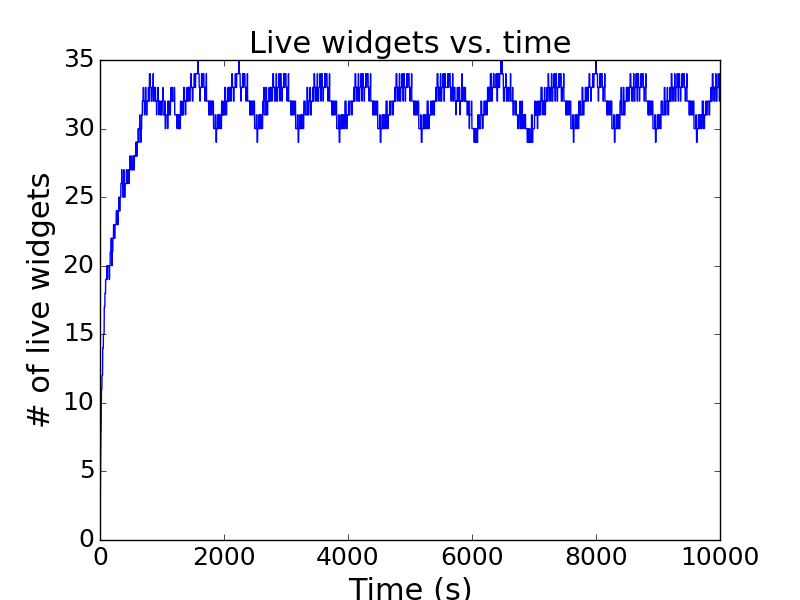
\includegraphics[width=0.99\columnwidth]{Figures/b2-total-widgets}
%\vspace{-\baselineskip}
\caption{Total alive widgets in the plant.}
\label{fig:linear_total_widgets}
        %\vspace{-\baselineskip}
    \end{subfigure}
    %\vspace{-\baselineskip}
    \caption{Experiment results for the plant shown in Figure~\ref{fig:linear_plant_graph}.}
    \label{fig:linear_model_exp}
    %\vspace{-1\baselineskip}
\end{figure*}



\begin{figure*}[!t]
\centering
    \begin{subfigure}[t]{0.33\linewidth}
        \centering
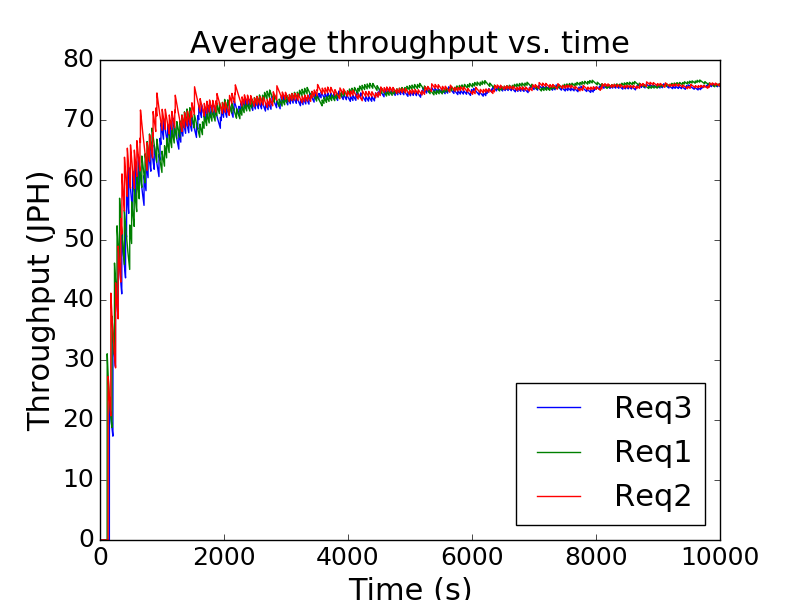
\includegraphics[width=0.99\columnwidth]{Figures/b3-throughput}
%\vspace{-\baselineskip}
\caption{Throughput of each widget (JPH).}
\label{fig:linear_plus_jph}
%\vspace{-1\baselineskip}
    \end{subfigure}%
        ~%\hspace{0.5cm} 
    \begin{subfigure}[t]{0.33\linewidth}
        \centering     
        %\vspace{3\baselineskip}     
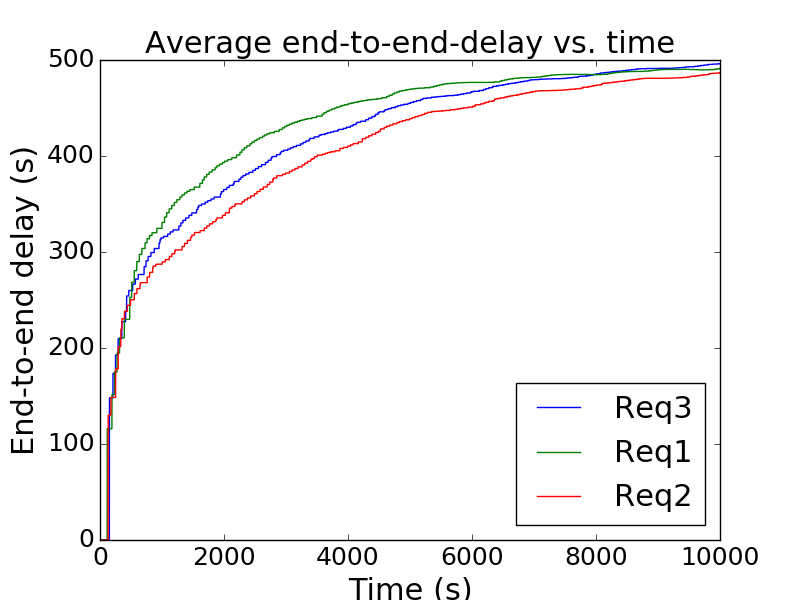
\includegraphics[width=0.99\columnwidth]{Figures/b3-end-to-end}
%\vspace{-\baselineskip}
\caption{End-to-end time of each widget.}
\label{fig:linear_plus_end_to_end}
    \end{subfigure}%
        ~ 
    \begin{subfigure}[t]{0.33\linewidth}
        \centering     
 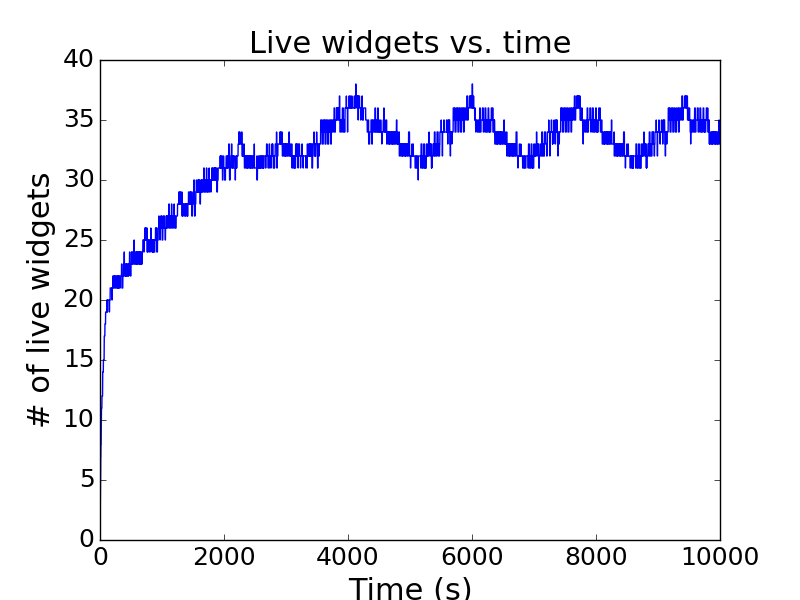
\includegraphics[width=0.99\columnwidth]{Figures/b3-total-widgets}
%\vspace{-\baselineskip}
\caption{Total alive widgets in the plant.}
\label{fig:linear_plus_total_widgets}
        %\vspace{-\baselineskip}
    \end{subfigure}
    %\vspace{-\baselineskip}
    \caption{Experiment results for the plant that has an additional cell, $v_6$, as shown in Figure~\ref{fig:linear_plant_plus_graph}.}
    \label{fig:linear_plus_exp}
    %\vspace{-1\baselineskip}
\end{figure*}

\section{Case Study}
\label{sec:case_study}
In this section we use a synthetic linear model and its variant as examples to demonstrate the use of the \mfname modeling framework.
We also carry out analysis using the simulator described in Section~\ref{sec:simulation}.

\subsection{A Synthetic Linear Model}
\label{subsec:linear_model}
Let's consider a simple linear manufacturing system consisting of five cells, $V=\{v_1,v_2,v_3,v_4,v_5\}$.
This plant contains a fork that provides multiple path options for dynamic allocation and support for fabricating multiple types of widgets.
The plant is represented as a graph (Figure~\ref{fig:linear_plant_graph}).
The supported operations and the time for each node to complete the designated operation is:\\

\begingroup
\setlength\parindent{24pt}
\indent $v_1 \colon \ T(v_1,op_1)=10s$\\
\indent $v_2 \colon \ T(v_2,op_2)=20s$\\
\indent $v_3 \colon \ T(v_3,op_3)=40s,\ T(v_3,op_4)=35s$\\
\indent $v_4 \colon \ T(v_4,op_5)=50s$\\
\indent $v_5 \colon \ T(v_5,op_6)=15s$\\
\endgroup





Let's consider three types of widgets to be fabricated in this plant, denoted by $\mathcal{R}=\{R_1,R_2,R_3\}$.
These requirements are listed in Table~\ref{tab:linear_plant_requirements}.
Requirement 1 is a typical linear manufacturing process that requires the widgets to visit the cells that support the corresponding operations in the given order.
Requirement 2 shows a different set of operations potentially requiring some cells to be bypassed.
For example, the path satisfying $R_2$ in the given plant is $\verttop \ra v_1 \ra v_2 \ra v_4 \ra v_5 \ra \vertbot$ where $v_1$ and $v_5$ do nothing to the widgets under this requirement.
Requirement 3 has an option for the system to choose a path that satisfies one of the operation requirements (\ie either $op_4$ or $op_5$ at the second stage).
These types of requirements are not uncommon since different models of machines can perform the same work on the widgets albeit with different tools.

\begin{table}[t]
\centering
\caption{Operational requirements for the linear model.}
\label{tab:linear_plant_requirements}
\begin{tabular}{|c|l|}
\hline
 & \multicolumn{1}{c|}{Operations}            \\ \hline \hline
$R_1$         & $op_1 \ra op_2 \ra op_3 \ra op_6$ \\ \hline
$R_2$         & $op_2 \ra op_5$  \\ \hline
$R_3$         & $op_1 \ra (op_4\ or\ op_5) \ra op_6$  \\ \hline
\end{tabular}
\end{table} 



The above plant and requirements are converted into YAML files as input for the simulator.
In the simulation, one widget is placed at the entrance (\ie $\verttop)$ in every tick, as introduced in Section~\ref{sec:simulation}. 
Each widget appearing at the entrance is assigned a requirement from $\{R_1, R_2, R_3\}$ in a round-robin fashion. 
We run the simulation for 10000 ticks (we assume that each tick represents one second in this experiment).
The simulation results are shown in Figure~\ref{fig:linear_model_exp}.%Figure~\ref{fig:linear_jph}, \ref{fig:linear_total_widgets} and \ref{fig:linear_end_to_end}.


The results suggest that the throughput stabilizes after $5000$ ticks.
The throughput for all three requirements converges to around $50 JPH$ to $60 JPH$ ($JPH$ stands for jobs-per-hour which is a common metric in manufacturing systems). 
Although the arrival rate of the widgets can potentially be higher (because one widget is introduced into the system at every tick, the maximum arrival rate is $3600/hour$ for three requirements and $1200/hour$ for each requirement),
the actual throughput is constrained by the bottleneck at $v_4$ with $op_5$ that takes 50s to complete the operation.
Hence, the throughput upper bound on this node is $(1/50)/3600=55.6JPH$.
As it is a mandatory hop for $R_2$, the throughput of the nodes and edges on the path for $R_2$ before this $v_4$ is also limited by its throughput $55.6JPH$.



\subsection{A Variant Model}
From the previous example, we observe that the throughput is constrained by $v_4$.
A reasonable method to further increase the throughput is to add another cell that supports the same operation, $op_5$.
Here, we consider the case that an additional cell with the same capability as $v_4$ is added as $v_6$.
The updated plant is shown as a graph in Figures~\ref{fig:linear_plant_plus_graph}.


\begin{figure}[h]
\begin{center}
	\resizebox{0.4\textwidth}{!}{%
 		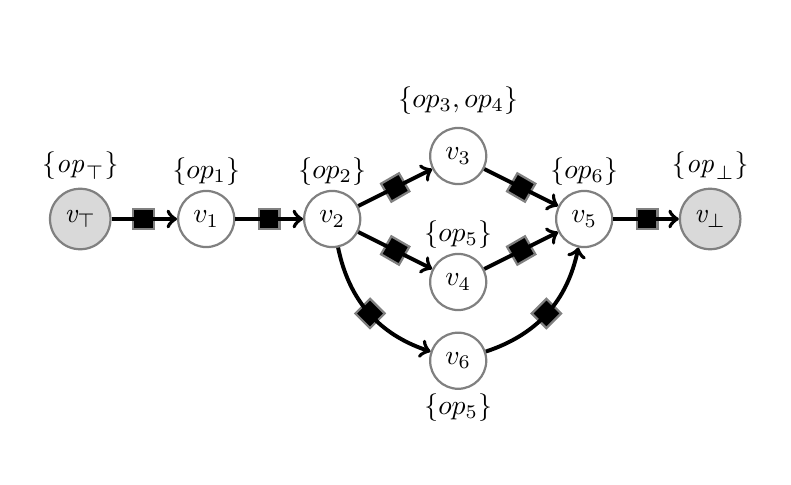
\begin{tikzpicture} 
 %[scale=.8,auto=left,every node/.style={circle,fill=blue!20}]
             [scale=.8,auto=left,every node/.style={circle,draw=black!50, thick},every path/.style={line width=0.5mm}]
 			\node[circle, fill=gray!30,label={[xshift=0cm, yshift=-0.4cm]$\{\optop\}$}] (v_t) at (-5,0) {$\verttop$};
             \node[label={[xshift=0cm, yshift=-0.4cm]$\{op_1\}$}] (v_1) at (-3,0) {$v_1$};
             \node[label={[xshift=0cm, yshift=-0.4cm]$\{op_2\}$}] (v_2) at (-1,0) {$v_2$};
             \node[label={[xshift=0cm, yshift=-0.6cm]$\{op_3,op_4\}$}] (v_3) at (1,1) {$v_3$};
             \node[label={[xshift=0cm, yshift=-0.4cm]$\{op_5\}$}] (v_4) at (1,-1) {$v_4$};
             \node[label={[xshift=0cm, yshift=-0.4cm]$\{op_6\}$}] (v_5) at (3,0) {$v_5$};  
             \node[label={[xshift=0cm, yshift=-1.6cm]$\{op_5\}$}] (v_6) at (1,-2.25) {$v_6$};                          
 			\node[circle, fill=gray!30,label={[xshift=0cm, yshift=-0.4cm]$\{\opbot\}$}] (v_b) at (5,0) {$\vertbot$};

			\node[rectangle,fill=black,minimum size=7.5pt] (v_c) at (-4,0) {};			
			\node[rectangle,fill=black,minimum size=7.5pt] (v_c) at (-2,0) {};
			\node[rectangle,fill=black,minimum size=7.5pt,rotate=30] (v_c) at (0,0.5) {};             
			\node[rectangle,fill=black,minimum size=7.5pt,rotate=60] (v_c) at (0,-0.5) {};          
			\node[rectangle,fill=black,minimum size=7.5pt,rotate=60] (v_c) at (2,0.5) {};  
			\node[rectangle,fill=black,minimum size=7.5pt,rotate=30] (v_c) at (2,-0.5) {}; 
			\node[rectangle,fill=black,minimum size=7.5pt] (v_c) at (4,0) {}; 	
			\node[rectangle,fill=black,minimum size=7.5pt] (v_c) at (-2,0) {};  
			\node[rectangle,fill=black,minimum size=7.5pt,rotate=45] (v_c) at (-0.4,-1.5) {};
			\node[rectangle,fill=black,minimum size=7.5pt,rotate=45] (v_c) at (2.4,-1.5) {};			
			
 			\path (v_t) edge[->] (v_1);
 			\path (v_1) edge[->] (v_2);
 			\path (v_2) edge[->] (v_3);
 			\path (v_2) edge[->] (v_4); 
 			\path (v_3) edge[->] (v_5); 						
 			\path (v_4) edge[->] (v_5);
 			\path (v_5) edge[->] (v_b);
 			
 			\path[]
            	(v_2) edge[->,bend right] (v_6)
                (v_6) edge[->,bend right] (v_5);
 		\end{tikzpicture}
	 	}
 	\end{center}
\caption{The graph for the plant introduced in Section~\ref{subsec:linear_model} with an additional cell, $v_6$, added.}
\label{fig:linear_plant_plus_graph}
\end{figure}


The plant with $v_6$ is then fed into the simulator for the experiment.
We keep the set of requirements and other configurations the same as the previous case for comparison.
The results are shown in Figure~\ref{fig:linear_plus_exp}.%Figures~\ref{fig:linear_plus_jph}, \ref{fig:linear_plus_total_widgets} and \ref{fig:linear_plus_end_to_end}.


From the simulation, we can observe that the throughput for all three requirements increases since the original bottleneck is removed after adding additional supports for $op_5$.
As a result, the end-to-end time for $R_2$ (\ie the requirement that requires $op_5$) decreases significantly.
Also, the total alive widgets slightly grow in this case because the capacity (\ie additional space for widgets to sit in) of the plant increases when the additional cell is added.
It's worth noting that $v_3$ becomes the new bottleneck in this setup as its support for $op_3$ has the highest time cost, which causes the congestion on the route to it.

\section{Conclusion}
\label{sec::concl}

Future manufacturing systems will be composed of complex
software and manufacturing plants that work in close coordination 
with each other. They will have to deal with failure, changing requirements,
security threats, \etc Hence, a system that has a {\em global} view
of the overall system will be invaluable for managing such systems. The
\mfname presented in this paper provides a mechanism for modeling and analysis of such systems. 
We envision that  it will engender a new set of research problems in 
 synthesis, verification, monitoring, fault-tolerance targeting 
 manufacturing and more general software-defined control systems. 
%  and build fault-tolerance mechanisms as well as
%security protocols in a seamless fashion. Manufacturing systems of the future
%will hence, be better managed, more efficient and agile.


%\subsection*{Acknowledgements}


%\pagebreak
%\newpage
%\IEEEtriggeratref{10}
%\bibliographystyle{plain}
\bibliographystyle{IEEEtran}
%\bibliographystyle{abbrv}
%\bibliographystyle{ACM-Reference-Format}

\bibliography{ref,sayan1,routing,dawnrefs,miguel-refs,morerefs,sibin.sdn,sibin.sdc}

\end{document}
